\pagestyle{mystyle}

\part{理论基础与背景}

\renewcommand{\parttitle}{理论基础与背景}

\chapter{绪论}

\section{引力波天文学的历史与发展}

引力波的存在是爱因斯坦广义相对论的核心预言之一。1916年，爱因斯坦在建立广义相对论后不久便指出，质量的加速运动会在时空中激起涟漪，以光速向外传播——这便是引力波。然而，由于引力波与物质的耦合极其微弱，其直接探测在此后近一个世纪内都被认为是遥不可及的目标。

间接证据首先来自脉冲双星系统。1974年，Hulse 和 Taylor 发现了第一个脉冲双星 PSR B1913+16，随后数十年的轨道周期观测表明，该系统的轨道能量损失与广义相对论预言的引力波辐射高度吻合~\cite{HulseTaylor1975}。这一发现使 Hulse 和 Taylor 获得了1993年的诺贝尔物理学奖，也坚定了物理学界直接探测引力波的信心。

\textbf{Hulse-Taylor 脉冲双星的发现经过}。
1974年11月，年仅24岁的博士研究生 Russell Hulse 在位于波多黎各的阿雷西博射电天文台执行一项系统性脉冲星巡天任务。他使用口径305米的球面射电望远镜，以1.4 GHz 频段对数百个天区进行重复扫描，目标是寻找射电脉冲星候选体并精确测定其脉冲周期。在当年7月至12月间，Hulse 共发现了40颗新脉冲星候选体，其中 PSR B1913+16 因一个异常现象引起了他的高度注意：该脉冲星的脉冲周期并非固定不变，而是以约7.75小时为周期做规律性振荡，振幅约为80微秒。这一周期性变化揭示了一个明确的物理机制——多普勒效应：PSR B1913+16 与一个看不见的伴星组成了一个绕转双星系统，脉冲星的周期性蓝移和红移对应其在轨道上朝向或背离地球的运动。

Hulse 将这一发现报告给其导师 Joseph Taylor，两人随即展开了系统性的后续观测。通过对脉冲到达时间（TOA，time of arrival）的精密测量，他们逐步重建出轨道参数：轨道周期约为7小时45分钟，轨道偏心率约为0.617（高度椭圆轨道），轨道半长轴约为1.95个太阳半径——这意味着整个双星系统可以装进我们太阳的半径之内。最重要的是，精确测定轨道参数后，广义相对论的广义后牛顿效应（施瓦西进动、时间膨胀、测地线进动）均可以得到精确检验。

从1974年到1982年，Taylor 团队持续积累 PSR B1913+16 的脉冲到达时间数据，时间跨度长达八年。在精密计时分析中，他们发现了一个关键现象：轨道周期以每年约76微秒的速率减小，即轨道在引力波辐射能量损失的驱动下缓慢衰减。将这一衰减速率与广义相对论对同等参数双星系统的预言相比较，两者吻合程度优于0.3\%，误差范围内与理论完全一致。这是引力波存在的第一个间接实验证据，被誉为“人类第一次感知到引力波”。此后的持续观测进一步将符合精度提升至万分之一量级，成为精度最高的引力波间接探测结果之一。

直接探测的突破发生在2015年9月14日。美国激光干涉引力波天文台（LIGO）的两台探测器几乎同时记录到一个持续约0.2秒的信号，经过严格的数据分析，确认这是来自约13亿光年外两个黑洞并合产生的引力波事件 GW150914~\cite{Abbott2016GW150914}。这一发现不仅直接验证了广义相对论在强场动力学条件下的预言，更开创了引力波天文学这一全新的天文学分支，使 Weiss、Barish 和 Thorne 获得了2017年的诺贝尔物理学奖。Advanced LIGO 的建设~\cite{LIGOScientific2015detector}和 Advanced Virgo 的加入~\cite{Acernese2015Virgo}，使三台探测器联合网络成为引力波天文学的核心基础设施。

\textbf{LIGO 的建设历程}。
激光干涉引力波天文台（LIGO）的诞生，是科学史上罕见的长期愿景与坚持不懈的典范。早在1972年，麻省理工学院（MIT）的 Rainer Weiss 就在一份内部报告中详细分析了激光干涉仪探测引力波的可行性，给出了主要噪声源的定量估计，奠定了现代引力波探测器的设计框架。1984年，Weiss、加州理工学院（Caltech）的 Kip Thorne 和 Ron Drever 正式向美国国家科学基金会（NSF）提交建设 LIGO 的方案，提出在两个地点分别建造臂长4公里的L型激光干涉仪，通过两台探测器的耦合（coincidence）分析来抑制局部噪声干扰。

1994年，LIGO 项目正式破土动工，选定路易斯安那州利文斯顿（Livingston）和华盛顿州汉福德（Hanford）两处地点。两个台址间距约3000公里，信号经过这一距离传播的时延约10毫秒，为耦合分析提供了重要约束。建设历时约六年，2002年，初代 LIGO（Initial LIGO，iLIGO）完成调试并正式开始科学运行，灵敏度在100 Hz 处达到约 $10^{-21}/\sqrt{\text{Hz}}$ 量级。2005年至2010年间，iLIGO 完成了 S1 至 S6 共六轮科学运行，未发现引力波信号，但对各类波源给出了重要的上限约束，同时大量积累了关于探测器性能与噪声源的宝贵经验。

2010年至2015年，LIGO 经历了全面的升级改造，成为 Advanced LIGO（aLIGO）。这次升级的核心技术改进包括：激光功率从初代的10 W 提升至 200 W，臂腔功率通过功率循环腔达到约750 kW；引入信号循环腔（signal recycling cavity），允许对特定频率的引力波信号进行共振增强；将悬挂系统由金属丝改为熔融石英纤维（fused silica），大幅降低热噪声；引入全新的四级悬挂隔振系统（quad pendulum seismic isolation），将地震噪声在10 Hz 以上频段衰减超过十个量级；探测器应变灵敏度比 iLIGO 提升约十倍，在 100 Hz 处达到约 $10^{-23}/\sqrt{\text{Hz}}$，在 LIGO 引力波天文学中实现了从“上限”到“探测”的历史性跨越。2015年9月，完成升级后不久的 Advanced LIGO 正式开始第一轮科学运行（O1），随即在运行仅两天后便捕获了人类历史上第一个引力波信号 GW150914。

\textbf{GW150914 的详细物理图像}。
GW150914 是引力波天文学史上最重要的单一事件，其每一个观测细节都承载着深刻的物理意义。信号在北京时间2015年9月14日17时50分45秒（UTC 09:50:45）被 Hanford 和 Livingston 两台探测器先后探测到，两台探测器的触发时延约为7毫秒，与光速传播3000公里的时延（约10毫秒）一致，方向性约束指向南半球天区。

从信号形态看，GW150914 是一个典型的啁啾信号：频率从约35 Hz 单调增加到约150 Hz，历时约0.2秒，随后以极快速度达到峰值振幅，然后在约0.05秒内衰减为零。这一时频演化轨迹与双黑洞并合的旋进-并合-衰荡三阶段模型高度吻合。峰值应变约为 $10^{-21}$，对于 LIGO 4公里臂长而言，对应的实际臂长变化约为 $4\times10^{-18}$ 米，约为质子半径（$\sim 10^{-15}$ m）的千分之四。Livingston 探测器的信噪比约为23.4，Hanford 探测器的信噪比约为13.0，两台探测器联合网络信噪比约为24.4。经过严格的背景估计和统计检验，GW150914 的显著性超过5.1$\sigma$，对应的误报率约为每20万年一次，以压倒性的统计证据确认了引力波的直接探测。

对波形的贝叶斯参数估计给出：啁啾质量 $\mathcal{M} \approx 28.3^{+1.8}_{-1.5}\,M_\odot$，两个黑洞的质量分别约为 $36.2^{+5.2}_{-3.8}\,M_\odot$ 和 $29.1^{+3.7}_{-4.4}\,M_\odot$，并合后残余黑洞质量约为 $62\,M_\odot$，缺失的约 $3\,M_\odot$ 以引力波的形式辐射。光度距离约为 $410^{+160}_{-180}$ Mpc（约13亿光年），对应红移 $z\approx0.09$。这是人类首次通过引力波直接观测到双黑洞并合，首次直接确认恒星级双黑洞系统的存在，并以直接实验方式检验了广义相对论在强场高速域的预言。

\textbf{O1--O4 观测轮次的科学成果}。
GW150914 的发现开启了引力波天文学的系统性观测时代。LIGO-Virgo-KAGRA 合作组此后相继完成了四轮科学观测，每一轮都带来了新的突破。第一轮观测（O1，2015年9月至2016年1月）历时约4个月，除 GW150914 外还探测到 GW151226（两个约14和8个太阳质量的黑洞并合）和 GW151012，共3个引力波事件候选体（其中GW150914和GW151226超过5$\sigma$显著性阈值，GW151012置信度稍低），初步确立了恒星级双黑洞并合的统计特征。

第二轮观测（O2，2016年11月至2017年8月）引入了欧洲 Virgo 探测器的加入，形成三台探测器的联合网络，显著提升了天空定位精度。O2 期间共探测到11个事件，最具里程碑意义的是2017年8月17日的双中子星并合事件 GW170817。该事件被引力波探测器、伽马射线望远镜（Fermi 和 INTEGRAL）、以及数十台光学、射电、X射线望远镜同步观测，是人类历史上首次实现的引力波与电磁波多信使联合观测，标志着多信使天文学新时代的正式开启。GW170817 距地球仅约40 Mpc，提供了迄今最精确的中子星参数约束，并独立测量了哈勃常数。

第三轮观测（O3，2019年4月至2020年3月）带来了引力波探测数量的大幅增加。O3 期间共探测到近百个引力波事件候选体，最终发布的 GWTC-3 引力波事件目录~\cite{Abbott2021GWTC3}包含90个置信度不等的候选体，覆盖双黑洞（BBH）、双中子星（BNS）、黑洞-中子星（NSBH）等多种类型，以及若干处于“质量间隙”的神秘天体。O3 还首次探测到质量超过100个太阳质量的黑洞（中间质量黑洞）候选体 GW190521，引发了关于黑洞形成机制的广泛讨论。第四轮观测（O4）于2023年5月开始、2025年11月结束，O4a 目录已经显著扩展公开样本规模；随着 O4 后续数据产品的发布，引力波天文学正在从“单次发现”迈向“海量统计”的大数据时代。

\subsection{激光干涉仪的工作原理}

LIGO/Virgo/KAGRA 等地面引力波探测器的核心是迈克尔逊激光干涉仪。其基本原理是：当引力波通过时，时空的伸缩会导致干涉仪两臂的光程差发生变化，从而改变干涉条纹的亮度。对于臂长为 $L$ 的干涉仪，引力波应变 $h$ 引起的臂长变化为
\begin{equation}
  \delta L = \frac{1}{2} h L,
\end{equation}
对于 LIGO（$L = 4$ km）和典型的引力波应变（$h \sim 10^{-21}$），臂长变化约为 $\delta L \sim 10^{-18}$ m，约为质子半径（$\sim 10^{-15}$ m）的千分之一量级。

为达到如此极端的测量精度，Advanced LIGO 采用了多项关键技术：功率循环腔（power recycling cavity）将激光功率从输入的约 200 W 提升至臂腔内的约 750 kW，增强光子散粒噪声的信噪比；信号循环腔（signal recycling cavity）对特定频率的引力波信号进行共振增强；法布里-珀罗臂腔（Fabry-Pérot arm cavity）使光束在臂中往返约 150 次，等效地将臂长增加至约 1200 km；以及主动隔振系统（active seismic isolation），将地震噪声在 10 Hz 以上频段衰减超过 10 个量级。

这些技术进步的背后是数十年的持续攻关。臂腔的精细度（finesse）约为450，对应光束在臂中平均往返约143次，使臂腔内循环光功率达到约750 kW，极大增强了光子数统计，将量子散粒噪声降低至约 $4\times10^{-24}/\sqrt{\text{Hz}}$（在100 Hz 处）。信号循环腔的引入在技术上称为“共振边带提取”（resonant sideband extraction），它改变了信号带宽，使探测器对特定引力波频率的灵敏度得到显著增强，同时配合压缩光（squeezed light）注入技术，可将散粒噪声进一步降低3 dB（Advanced LIGO O3 已实现这一技术突破）。四级悬挂隔振系统的最底级采用熔融石英纤维支撑镜面，纤维的极低机械损耗将镜面热噪声降至最低水平，使100 Hz 频段的热噪声贡献不超过散粒噪声。

探测器的灵敏度受三类基本噪声限制：低频段（$\lesssim 10$ Hz）由地震噪声和重力梯度噪声主导；中频段（约 10--200 Hz）由热噪声（悬挂系统和镜面涂层的布朗运动）主导；高频段（$\gtrsim 200$ Hz）由量子散粒噪声（光子到达的泊松统计涨落）主导。这三类噪声的频率特性共同决定了探测器的灵敏度曲线 $S_n(f)$，也直接影响了匹配滤波和机器学习方法的设计选择。

重力梯度噪声（Gravity Gradient Noise / Newtonian Noise，GGN/NN）是地面引力波探测器低频灵敏度的根本性限制。地表附近的密度涨落——无论是地震波引起的地面形变还是大气压力变化——都会产生引力梯度，直接作用于检验质量，这一干扰无法通过机械隔振消除，只能通过在检验质量周围布置密集的传感器网络来测量并在线减除。正是这一根本性限制，促使下一代探测器（如爱因斯坦望远镜 ET 和日本的 KAGRA）选择建于地下，利用岩层的天然衰减将地震噪声降低两到三个量级。

\subsection{引力波观测的科学贡献}

在所有宇宙信使中，引力波最特殊的地方在于，它不依赖物质辐射的再加工，而是直接记录致密天体附近时空几何的动态变化。电磁波告诉我们物质如何发光，中微子告诉我们弱相互作用过程如何释放能量；引力波则把黑洞视界附近、致密星内部和宇宙早期的动力学过程转化为可测量的时空应变。它因此为现代天文学提供了一种前所未有的观测方式：我们不仅可以“看见”光与粒子，还可以“听见”引力如何在极端条件下传播、叠加并重塑时空。

这种信使的独特性，使引力波观测天然连接了现代科学大厦中的若干“乌云”级问题。强场引力是否严格遵从广义相对论？黑洞是否完全由质量、电荷和自旋刻画？恒星级黑洞的质量谱为什么具有峰值和间隙？中子星内部的冷致密核物质状态方程究竟如何？哈勃张力是否暗示系统误差之外的新物理？宇宙早期相变、宇宙弦或暗物质环境是否在随机引力波背景中留下痕迹？这些问题分属基础物理、天体物理、核物理和宇宙学，但都可以通过引力波观测获得独立约束。

\textbf{基础物理}：引力波波形直接编码强场、高速和强非线性条件下的引力动力学。双黑洞并合的旋近、并合和衰荡阶段分别检验后牛顿动力学、强场非线性相互作用和黑洞准简正模；多信使事件中引力波与电磁信号的到达时延可约束引力波传播速度；高信噪比事件还可用于限制引力子质量、洛伦兹不变性破缺和广义相对论之外的极化模式。

\textbf{致密天体物理}：引力波事件目录（GWTC-3）揭示了双黑洞质量分布的复杂结构，发现了质量间隙（$\sim 3$--$5\,M_\odot$）中的候选天体，以及超出传统恒星演化预期的高质量黑洞（如 $\sim 85\,M_\odot$ 成分）~\cite{Abbott2021GWTC3}。这些观测对恒星演化、公共包层过程、动力学俘获、多代并合和致密星团环境提出了新的约束，使黑洞种群从理论假设转变为可统计检验的观测对象。

\textbf{多信使天文学与核物理}：GW170817 的多信使观测表明，双中子星并合不仅会产生引力波，还会伴随短伽马射线暴、千新星、X 射线与射电辐射~\cite{Abbott2017GW170817}。这一事件把引力波天文学推进到“引力波+电磁波”协同观测的新阶段，并从观测上连接了并合源、重元素 r 过程核合成与短伽马射线暴之间的因果链条。引力波相位中的潮汐形变率还把中子星状态方程问题推进到天体尺度，为极端密度下核物质的半径、可压缩性和最大质量提供了独特约束。

\textbf{宇宙学}：引力波事件提供了不依赖传统距离阶梯的“标准汽笛”距离测量。GW170817 已经给出哈勃常数的独立约束；随着双中子星事件、黑洞-中子星事件和“暗汽笛”统计样本的增长，引力波有望在哈勃张力、宇宙膨胀史和引力理论的宇宙学尺度检验中发挥越来越重要的作用~\cite{Jin2025GWStandardSirens}。未来空间探测器还将把观测窗口延伸到大质量黑洞并合和随机背景，为早期宇宙相变、宇宙弦和暗物质相关模型提供新的观测入口。

\section{国际与国内探测计划概览}

当前运行的地面引力波探测器构成了一个全球网络。美国的 Advanced LIGO 拥有两台探测器（Hanford 和 Livingston），臂长 4 公里，灵敏频段约 10 Hz--几千 Hz。欧洲的 Advanced Virgo 位于意大利，臂长 3 公里。日本的 KAGRA 是首台建于地下的低温引力波探测器，旨在进一步降低热噪声。印度的 LIGO-India 正在建设中，将进一步提升全球网络的天空定位能力。\textbf{2024年，中国科学院大学正式加入 LIGO 科学合作组织（LSC）}，成为 LSC 在中国大陆地区的成员单位之一，标志着中国地面引力波研究与国际顶级合作网络的深度融合。

地面探测器受限于地球尺度和地震噪声，灵敏频段通常在 10 Hz 以上，无法探测更低频率的引力波源。为此，多个空间引力波探测计划正在推进，它们共同把观测窗口延伸到毫赫兹频段：

\textbf{LISA}（Laser Interferometer Space Antenna）：欧洲航天局主导，三颗卫星组成等边三角形星座，臂长 250 万公里，目标工作频段主要面向毫赫兹窗口，预计2030年代发射~\cite{LISA2017proposal}。

\textbf{太极}（Taiji）：中国科学院主导，三颗卫星，臂长 300 万公里，与 LISA 频段相近，预计2030年代发射~\cite{Hu2017Taiji_NSR,Ruan2020Taiji_RiP,wang2024challenges}。

\textbf{天琴}（TianQin）：中山大学主导，三颗卫星绕地球运行，臂长约 17 万公里，灵敏度窗口同样面向毫赫兹附近的空间探测窗口，但峰值灵敏区域较 LISA/太极偏高，预计2030年代发射~\cite{Luo2016TianQin,Mei2021TianQin_PTEP}。

三个空间任务的联合观测将显著提升参数估计精度和天空定位能力，是未来空间引力波天文学的重要发展方向~\cite{du2026taiji}。

\subsection{下一代地面探测器}

当前的 Advanced LIGO/Virgo/KAGRA 网络代表了第二代地面引力波探测器的技术水平，其灵敏度在未来数年内仍有提升空间（A+ 和 AdV+ 升级计划），但根本性的突破将来自第三代探测器。

爱因斯坦望远镜（Einstein Telescope，ET）是欧洲提出的下一代地面引力波探测器~\cite{Punturo2010ET}，其设计理念在多个维度超越了现有技术。ET 采用等边三角形构型，三条臂各长10公里，三角形构型相比L型具有天然的优势：三个探测器通道可以通过线性组合分离引力波的两种极化分量，提供更完整的极化信息，同时三角形的几何结构使得全天空覆盖更均匀。ET 将建于地下约100至200米深处，利用岩层对地震噪声的天然衰减，突破地面探测器低频灵敏度的根本限制。在技术上，ET 计划采用低温镜面、高功率激光和频率相关量子压缩等技术，以同时降低热噪声和量子噪声。其设计目标是在约2--3 Hz 以上扩展地面探测器的低频观测能力，并在数十至数百 Hz 频段相对 Advanced LIGO 提升约一个量级的应变灵敏度。这将使 ET 能够探测高红移双黑洞并合事件，并显著提升对双中子星早期旋近、超新星核坍缩以及随机引力波背景的观测能力。

宇宙探索者（Cosmic Explorer，CE）是美国提出的下一代地面引力波探测器计划~\cite{Evans2021CE}，其核心思路是通过大幅增加臂长来提升灵敏度。CE 采用标准L型构型，臂长约40公里（是 Advanced LIGO 的10倍），这意味着在相同的应变灵敏度下，臂长变化的绝对量增加10倍，从而使探测信噪比大幅提升。CE 预计将建于地面，但通过超低噪声隔振系统和先进的量子技术，在5 Hz 至10 Hz 以上频段实现突破性灵敏度。CE 与 ET 的联合网络（“下一代网络”）将能够对宇宙学距离上的引力波事件进行完整的参数估计，并在有利事件上显著改善天空定位、距离和质量测量精度。这将使引力波成为精密宇宙学的重要标准汽笛工具，并为哈勃张力等问题提供独立观测约束；具体精度仍取决于事件样本、探测器网络配置和系统误差控制。

\subsection{空间引力波探测器的技术原理}

空间引力波探测器与地面探测器在工作原理上有本质相同之处——均基于激光干涉测量两个自由浮动检验质量之间距离的微小变化——但面临的技术挑战和实现方式存在根本差异。

LISA（Laser Interferometer Space Antenna）是由欧洲航天局（ESA）主导的空间引力波探测任务，其技术方案历经三十余年的演进。LISA 由三颗卫星构成等边三角形星座，边长250万公里，绕太阳运行，与地球保持约 $20°$ 的夹角，轨道倾角约 $60°$，使得星座平面相对黄道倾斜，以实现全天空扫描。每颗卫星内部包含两个检验质量（金铂合金立方体，边长约4.6厘米），悬浮于超高真空腔室中，通过微推进器主动维持无拖拽飞行（drag-free flight）——即卫星外壳精确跟随检验质量的自由落体轨迹，消除太阳风压力和太阳辐射压力等非引力干扰。LISA 的激光波长为1064 nm，激光功率约2 W，经过望远镜（口径约30 cm）发射后，到达250万公里外的另一颗卫星时功率约降至 pW 量级，因此 LISA 采用的不是传统的反射干涉，而是“转发”方案：接收方卫星用本地激光器进行外差干涉，再将相位信息发回。LISA 的位移噪声目标为约 $1\,\text{pm}/\sqrt{\text{Hz}}$（频率在 3 mHz 处），加速度噪声目标为约 $3 \times 10^{-15}\,\text{m/s}^2/\sqrt{\text{Hz}}$（低频处），这些指标已由2015至2017年在轨运行的 LISA Pathfinder 任务成功验证，其实测性能甚至超越了设计指标一个量级。

太极（Taiji）是中国科学院主导的空间引力波探测任务，在设计上与 LISA 高度相似但有若干差异。太极的臂长为300万公里，略长于 LISA，这使其在中低频段（约 $1\,\text{mHz}$）的灵敏度略优于 LISA。太极的三颗卫星质量约为550公斤，激光功率2 W，望远镜口径300毫米，位移噪声目标 $1\,\text{pm}/\sqrt{\text{Hz}}$，加速度噪声目标 $3 \times 10^{-15}\,\text{m/s}^2/\sqrt{\text{Hz}}$。太极的轨道设计与 LISA 不同，采用绕太阳的日心轨道，与地球保持约 $20°$ 夹角，星座平面相对黄道倾角约为 $18°$，这一差异使太极与 LISA 具有不同的天空灵敏度分布，因此两者的联合观测将大幅提升天空定位能力。太极计划分三步走：太极-1（2019年发射）用于在轨技术验证；太极-2为单星验证；太极-3（预计2030年代）为三星正式科学任务。

天琴（TianQin）是中山大学主导的空间引力波探测任务，其轨道设计与 LISA/太极有根本性差异。天琴采用绕地球的高轨道，三颗卫星位于距地约10万公里的近圆轨道，臂长约17万公里，轨道平面垂直于指向白矮星双星系统 RX J0806.3+1527（天琴的“参考源”）的方向。这一设计的优点是轨道较低、通讯时延短，且与地面站的联系更紧密；缺点是臂长较短（比 LISA 短约14倍），因此峰值灵敏度更偏向毫赫兹窗口的高频端，对超大质量黑洞并合信号的覆盖略弱于 LISA/太极，但对部分银河系双星、恒星质量双黑洞早期旋近以及中等质量黑洞相关信号仍然具有重要科学价值。天琴的科学目标还包括验证弱等效原理（精度达 $10^{-8}$）和精密测量地球引力场，体现了科学目标的多元性。

三个空间任务的科学合作愿景已有明确的技术论证。LISA-太极联合网络（LISA + Taiji）由于两者轨道平面之间存在夹角，联合观测可将 MBHB 的天空定位精度从单任务的约 $10\,\text{deg}^2$ 提升至约 $0.1\,\text{deg}^2$，这对于引力波与电磁对应体的关联搜索至关重要。LISA-太极-天琴三星网络进一步增加了基线，理论上可将某些 EMRI 事件的参数测量精度再提升一到两个量级。这种多任务协同观测的范式，也对数据分析方法提出了全新需求：如何从多个独立数据流中联合提取信号、处理相关噪声、以及在全局拟合框架下同时优化多个探测器的参数推断，是本书后续章节方法研究的重要动机之一。

\section{引力波数据分析的任务层次与挑战}

引力波物理学家伯纳德·舒尔茨（Bernard Schutz）曾系统归纳成功观测引力波的五条关键要素：（1）良好的探测器技术；（2）良好的波形模板；（3）良好的数据分析方法和技术；（4）多个独立探测器间的一致性观测；（5）引力波天文学和电磁波天文学的一致性观测。这五条要素不仅描述了探测成功的条件，也定义了引力波数据分析研究的核心使命。其中要素（2）至（4）尤其强调数据本身及其分析方法的重要性：波形模板决定“要在数据中寻找什么”，分析技术决定“如何从噪声中提取证据”，多探测器一致性观测则决定“候选信号是否能经受独立数据流的交叉检验”。这三者共同构成本书研究主线中最直接的方法论基础。

引力波数据分析的核心任务可以分为三个层次：

\textbf{信号搜索与探测}：从探测器输出的含噪数据中判断是否存在引力波信号，并确定信号的大致时间和参数范围。这是数据分析链条的第一步，要求在保持高探测率的同时将误报率控制在可接受水平。

\textbf{参数估计}：对已探测到的信号，推断引力波源的物理参数（质量、自旋、距离、天空位置等）的后验概率分布。这是提取引力波天文学科学价值的核心步骤，要求在高维参数空间中进行精确的贝叶斯推断。

这三个层次的任务在科学目标和技术挑战上密切关联，但在方法论上各有侧重。信号搜索追求高灵敏度（最大化探测率）和低误报率（最小化假阳性），是一个统计检验问题，以奈曼-皮尔逊最优性为理论基础；参数估计追求后验分布的精确性和完整性（正确量化不确定度），是一个贝叶斯推断问题，以贝叶斯定理为理论基础；天体物理与宇宙学推断追求对种群统计规律的无偏提取，是一个层次贝叶斯问题，需要对探测选择效应（detection selection effects）进行显式修正。三个层次的相互衔接——搜索给参数估计提供输入，参数估计给宇宙学推断提供输入——构成了引力波数据分析管道的整体结构。AI方法在这三个层次上分别有不同的作用：在搜索层次，AI方法加速触发生成并提升glitch鉴别能力；在参数估计层次，SBI方法压缩推断时间；在宇宙学推断层次，深度学习的表征学习能力有助于捕捉种群参数的复杂依赖关系。

\textbf{天体物理与宇宙学推断}：基于引力波事件的统计样本，推断致密天体的形成与演化、宇宙学参数（如哈勃常数）、以及基础物理（广义相对论检验、暗物质约束等）。

这三个层次的任务面临共同的挑战：引力波信号极其微弱（地面探测器的应变灵敏度约为 $10^{-23}$），淹没在比信号强数个量级的噪声中；探测器噪声具有非高斯、非平稳的复杂特性；参数空间维度高（双黑洞系统约 15 维，EMRI 系统约 17 维），且存在强参数简并；空间引力波探测器还面临数百万个信号同时叠加的全局拟合挑战~\cite{wang2024challenges}。

\subsection{信号搜索的具体挑战}

引力波信号搜索的核心困难在于极端的信噪比条件与复杂的噪声环境的叠加。在地面探测器中，典型的引力波应变约为 $10^{-23}$，而量子散粒噪声在100 Hz 处约为 $2\times10^{-24}/\sqrt{\text{Hz}}$，对于持续约1秒的信号，有效信噪比约为10。这意味着信号功率仅为噪声功率的约百分之一，在时域波形上几乎完全不可见，必须依赖匹配滤波等相干积分方法才能从噪声中提取。

然而，真实探测器的噪声远比理想的高斯白噪声复杂。非高斯暂态噪声（glitch）是信号搜索中误报率的主要来源。在 Advanced LIGO 的典型运行状态下，每小时约有数个至数十个 glitch 事件，其中部分 glitch 的幅度可比背景噪声高出一到两个量级，持续时间从毫秒到数秒不等，形态多样。常见的 glitch 类型包括：持续时间约数毫秒、频率约100至300 Hz 的“blip”型 glitch（来源不明，可能与镜面散射光有关）；持续时间约数秒、频率从低到高扫描的“scattered light”型 glitch（来自散射光的干涉）；以及“koi fish”型、“tomte”型等数十种已命名的 glitch 类型。这些 glitch 在时频图上的形态有时与真实的引力波信号高度相似，是区分真实信号与噪声伪迹的核心挑战。

非平稳性是另一个根本性挑战。探测器的灵敏度随时间缓慢变化，在特定时段（如地震活动增强、激光功率波动、环境温度变化）会出现突发性的灵敏度下降。这种非平稳性导致基于固定噪声模型的统计方法失效：如果噪声功率谱在分析时段内发生了显著变化，基于旧噪声模型计算的信噪比将出现系统性偏差，导致误报率升高或探测率下降。实际的搜索流水线（如 PyCBC 和 GstLAL）需要实时估计和追踪噪声功率谱，通常采用滑动时间窗口的方法，但这引入了对非平稳性的时间尺度假设，在快速变化的噪声环境中仍然面临挑战。

参数空间的高维度使穷举搜索不可行。对于双黑洞系统，完整的参数空间包括两个天体的质量（2维）、自旋矢量（6维）、轨道倾角（2维）、天空位置（2维）、距离（1维）、并合时刻（1维）和初始相位（1维），共约15维。在匹配滤波框架下，需要构建足够密集的模板库，使得任意真实信号与最近模板之间的匹配度（fitting factor，FF）不低于约0.97。实际搜索通常通过解析极大化、参数降维和分区模板库设计来避免直接覆盖完整15维空间；即便如此，非自旋或对齐自旋双黑洞模板库也可达到 $10^4$ 至 $10^6$ 量级，若显式覆盖强进动和高阶模式效应，模板数量会进一步迅速膨胀。对于 EMRI 系统，参数空间约17维，且精确波形计算耗时，传统模板库方法难以直接承担，这正是机器学习方法在 EMRI 搜索与参数估计中具有重要价值的根本原因。

\subsection{参数估计的科学意义}

引力波参数估计不仅是数据分析的技术任务，更是提取引力波天文学科学价值的核心环节。精确的参数测量在多个科学方向上具有不可替代的意义。

在致密天体物理方面，精确的质量测量是约束黑洞形成机制和演化路径的关键。GWTC-3 中的双黑洞质量分布揭示了若干重要特征：在约 $10\,M_\odot$ 处存在一个质量峰，可能对应恒星演化中的特定质量损失机制；在约 $35\,M_\odot$ 处存在另一个峰，可能与对不稳定脉冲超新星（pulsational pair-instability supernova）有关；在约 $3\,M_\odot$ 至 $5\,M_\odot$ 的“质量间隙”中存在若干候选体，其起源（是中子星还是黑洞？）对核物理和超新星机制有重要约束。自旋参数的测量则可以区分黑洞的起源：孤立双星演化产生的黑洞自旋通常与轨道角动量对齐（有效自旋参数 $\chi_\text{eff} > 0$），而动力学俘获（如在球状星团中）产生的双黑洞自旋方向随机，$\chi_\text{eff}$ 的分布更宽且对称于零。

在宇宙学方面，引力波事件提供了独立于传统距离阶梯的哈勃常数测量方法。引力波信号的振幅直接给出光度距离，而无需任何标准烛光的校准；结合电磁对应体（如 GW170817 的宿主星系 NGC 4993）提供的红移，可以直接测量哈勃常数。这一方法被称为“标准汽笛”（standard siren），其精度随引力波事件数量、宿主星系关联质量和系统误差控制水平的提升而改善，有望为判断哈勃张力的来源提供独立信息。

在广义相对论检验方面，引力波波形的精确参数估计提供了强场动力学条件下的广义相对论检验。后牛顿参数的测量可以约束广义相对论的高阶修正项；衰荡阶段的准简正模频率和衰减时间可以检验“黑洞无毛定理”（即黑洞完全由质量和自旋描述）；引力波传播速度的测量（通过多信使时延）可以约束引力子质量和洛伦兹不变性破缺。这些检验的精度随信噪比的提升而改善，下一代探测器将把广义相对论检验的精度提升数个量级。

引力波参数估计的科学价值还体现在核物理方向。双中子星并合事件（BNS）的并合后动力学携带了关于中子星物质的信息：中子星的潮汐形变率（tidal deformability）$\Lambda$ 对引力波信号相位的贡献在并合前最后几个轨道周期内显著增大，通过精确测量 $\Lambda$ 可以约束中子星状态方程（equation of state，EOS）——即极端密度下核物质的压力-密度关系。GW170817 对 $\Lambda$ 的测量已经排除了一部分极硬状态方程，并将典型中子星半径约束到十余公里量级，是中子星内部物质性质研究的重要约束之一。中子星半径的精确测量——从引力波（潮汐形变）和 X 射线（热辐射）两个独立方向获得的约束的综合——将是多信使天文学最重要的科学产出之一，而高精度的 AI 参数估计方法（特别是 SBI 对包含物质效应的 BNS 波形的快速处理）是实现这一目标的关键使能技术。

天体物理与宇宙学推断层次的数据分析——从多个引力波事件的参数后验分布推断种群统计规律——代表了引力波天文学最高层次的科学目标，也对方法论提出了最高的要求。当引力波事件数量从当前的约90个增加到未来的约1000个（O5 期间预期）乃至 $10^5$ 个（爱因斯坦望远镜运行期间预期），传统的“逐事件参数估计→统计汇总”的两步方法将面临严重的计算瓶颈，而且逐步积累的系统误差也会在统计汇总中放大。面向未来的种群推断方法需要能够同时处理探测选择效应（detection selection bias——信噪比高的事件更容易被探测到，导致样本偏差）和参数估计不确定度的传播，这对于贝叶斯层次分析的效率和准确性提出了很高要求。SBI 方法的多事件联合推断能力（第6章）将在这一层次发挥核心作用，使天体物理种群分析能够实时响应不断增加的观测数据，成为引力波天文学走向“大数据科学”的关键使能技术。

空间引力波探测器面临的数据分析挑战在量级上远超地面探测器，其核心困难在于“全局拟合”问题。在 LISA/太极的灵敏频段内，同时存在的引力波信号数量可达数百万个：银河系内约有 $10^7$ 至 $10^8$ 个双白矮星系统，其中约 $10^4$ 至 $10^5$ 个在 LISA 频段内可分辨，其余形成不可分辨的混叠背景（confusion noise）；此外还有数十个 EMRI 事件、数个 MBHB 并合事件、以及随机引力波背景。这些信号在频域上高度重叠，无法逐一独立分析，必须在统一的框架下同时拟合所有信号和噪声参数，这就是“全局拟合”问题。

全局拟合的参数空间维度极高：每个可分辨的双白矮星有约7个参数，$10^4$ 个可分辨源对应约 $7\times10^4$ 维参数空间；每个 EMRI 有约17个参数；MBHB 有约15个参数；加上噪声参数和前景模型参数，总有效维度可达 $10^5$ 至 $10^7$ 量级，具体取决于任务时长、可分辨源数量和建模精度。传统的 MCMC 方法若直接作用于完整联合空间，收敛时间可能长到难以满足任务需求。这一挑战是本书第10章的核心主题，也是 AI 方法在空间引力波数据分析中具有重要价值的根本动机：机器学习方法（特别是模拟推断和深度生成模型）有望把全局拟合中的若干子问题从年级或月级计算压缩到天级乃至更短时间，从而使空间引力波天文学的准实时迭代分析更接近可行。

\subsection{数据分析的三层挑战：从信号识别到全局拟合}

上述三个任务层次——信号搜索、参数估计、天体物理推断——在方法论上构成递进关系，但每一层都面临独特的计算瓶颈，且这些瓶颈随探测器灵敏度的提升而急剧恶化。将三层挑战并置审视，有助于理解为何 AI 方法不是对传统方法的局部改良，而是整个数据分析范式的系统性重构。

\textbf{第一层：信号识别}。在噪声中检测引力波信号的存在，本质上是一个假设检验问题：在零假设（纯噪声）与备择假设（信号加噪声）之间做出判断。匹配滤波是奈曼-皮尔逊最优检验统计量，其信噪比定义为
\begin{equation}
\rho = \frac{(d | h)}{\sqrt{(h | h)}},
\end{equation}
其中 $(a|b) = 4\,\text{Re}\int_0^\infty \tilde{a}(f)\tilde{b}^*(f)/S_n(f)\,\mathrm{d}f$ 为噪声加权内积，$S_n(f)$ 为单边功率谱密度。匹配滤波的最优性依赖于两个前提：噪声为平稳高斯过程，且信号波形精确已知。在实际应用中，这两个前提均不严格成立，但匹配滤波仍是地面探测器信号搜索的核心工具。

匹配滤波的根本计算瓶颈在于模板库的规模。为覆盖参数空间中所有可能的信号，需要构建一个足够密集的模板网格，使得任意真实信号与最近模板的匹配度（fitting factor，FF）不低于约0.97。模板数量随参数空间维度和波形复杂度增加而快速增长：对于非自旋或对齐自旋双黑洞系统，模板库通常已达 $10^4$--$10^6$ 量级；若显式覆盖强进动、自旋高维结构或 EMRI 长时信号，直接模板库策略会遇到极高试验因子和计算代价。即便在当前双黑洞搜索中，大量模板与长时数据段的重复匹配滤波也会消耗可观计算资源。

机器学习方法在信号识别层次的核心优势在于推断速度。经过训练的卷积神经网络（CNN）或 Transformer 模型可以在毫秒量级内完成对一段数据的分类，而无需显式构建模板库。2021年举办的机器学习引力波搜索挑战赛（MLGWSC-1）对多种 AI 方法与传统匹配滤波流水线进行了系统性比较，结果表明：在相同误报率条件下，最优的机器学习方法的探测灵敏度约为传统方法的70\%，即存在约30\%的性能差距~\cite{schafer2023mlgwsc1}。这一差距揭示了当前 AI 方法在信号识别层次的局限性，也指明了未来改进的方向：如何在保持毫秒级推断速度的同时，将探测灵敏度提升至与匹配滤波相当的水平，是第5章的核心问题之一。

\textbf{第二层：参数估计}。推断引力波源物理参数的后验概率分布 $p(\boldsymbol{\theta}|d)$，是贝叶斯推断问题：
\begin{equation}
p(\boldsymbol{\theta}|d) \propto p(d|\boldsymbol{\theta})\,p(\boldsymbol{\theta}),
\end{equation}
其中似然函数 $p(d|\boldsymbol{\theta}) \propto \exp\!\left[-\frac{1}{2}(d - h(\boldsymbol{\theta})|d - h(\boldsymbol{\theta}))\right]$，$p(\boldsymbol{\theta})$ 为先验分布。由于似然函数的计算需要生成波形 $h(\boldsymbol{\theta})$，而后验分布在高维参数空间中具有复杂的多峰结构，传统的马尔可夫链蒙特卡洛（MCMC）方法需要对似然函数进行大量评估（通常为 $10^6$ 至 $10^8$ 次），每次评估需要生成一个波形（约毫秒至秒量级），导致单个事件的参数估计耗时从数小时（双黑洞）到数月（EMRI）不等。

模拟推断（SBI）方法通过训练神经网络直接近似后验分布，将推断时间从小时量级压缩至秒量级，实现了约 $10^6$ 倍的加速~\cite{Dax2021RNPE}。这一加速的代价是训练阶段的一次性计算投入（通常需要数天至数周的 GPU 计算），以及对波形模型的隐式依赖（训练数据的质量决定了推断精度的上限）。精度与速度的权衡是 SBI 方法的核心设计问题：如何在保证后验分布精度（特别是尾部行为和参数简并结构）的同时最大化推断速度，是第6章的核心主题。

\textbf{第三层：全局拟合}。空间引力波探测器的数据分析面临前两层挑战的叠加，并引入了本质上更困难的多源联合分析问题。在 LISA/太极的灵敏频段内，数万个可分辨信号在频域上高度重叠，无法逐一独立分析。全局拟合要求在约 $10^7$ 维的联合参数空间中同时推断所有信号和噪声参数，这一规模使得任何基于逐点似然评估的方法（包括 MCMC 和嵌套采样）在计算上不可行。

当前最有前景的策略是迭代减除（iterative subtraction）：先识别并拟合最强的信号，将其从数据中减除，再对残差数据重复上述过程，直至所有可分辨信号均被提取。这一策略的关键挑战在于误差传播：早期步骤的参数估计误差会在减除过程中积累，影响后续步骤的精度。AI 方法在全局拟合中的角色不再是对传统方法的加速替代，而是作为必要的基础设施：深度生成模型可以高效地近似高维联合后验分布，强化学习可以优化迭代减除的策略，而神经网络波形模型可以将 EMRI 等计算密集型波形的生成速度提升数个量级，使全局拟合在任务期内（约4至10年）完成成为可能。

三层挑战的共同主线是：随着探测器灵敏度和事件率的提升，传统方法的计算代价以超线性方式增长，而 AI 方法的推断代价（训练完成后）几乎与事件数量无关。这一根本性的计算经济学差异，是本书系统性引入 AI 方法的核心动机。

\subsection{计算资源与科学产出的矛盾：规模化挑战}

引力波天文学正在经历从“稀有事件天文学”向“大数据天文学”的范式转变。这一转变的驱动力是探测器灵敏度的持续提升和探测网络的扩展，其结果是引力波事件率、数据量和分析复杂度的同步指数增长，而现有的计算基础设施和分析方法论尚未为这一转变做好充分准备。

\textbf{事件率的快速增长}。LVK 第一次观测运行（O1，2015--2016年）探测到约3个引力波事件；第三次观测运行（O3，2019--2020年）发布了90个置信度不等的候选体；O4 进一步增加了公开候选样本，并把引力波天文学推向大样本统计阶段。下一代地面探测器爱因斯坦望远镜（ET）和宇宙探索者（CE）的灵敏度将比当前探测器提升约一个量级，预期年探测率可能达到 $10^4$--$10^5$ 量级，具体数值取决于天体物理事件率、探测网络配置和分析阈值。

这一事件率的增长对数据分析流水线提出了根本性挑战。在 O3 期间，单个引力波事件的参数估计通常需要数小时至数天，并依赖大量 CPU 核并行计算。若将相同的逐事件精密采样流程直接推广到 ET/CE 时代的大样本目录，计算需求将随事件数近似线性增长，并迅速超过常规人工逐事件分析模式能够承受的范围。自动化、高速的 AI 参数估计方法因此成为缓解这一瓶颈的关键技术路线之一。

\textbf{数据量与数据复杂度的增长}。地面探测器不仅记录主引力波应变通道，还持续记录大量辅助通道、环境监测通道和数据质量信息；用于公开科学分析的应变数据通常已经过筛选、标定和降采样，但低延迟管道仍需同时处理数据质量、噪声谱估计和候选触发背景。太极和 LISA 的主科学数据采样率较低，数据体量本身未必大于地面探测器；真正的困难在于多源叠加、时变响应、TDI 处理和全局拟合，使每单位数据所需的推断计算量显著增加。

实时处理的计算需求是另一个关键约束。引力波触发的多信使天文学要求在信号到达后数秒至数分钟内完成初步参数估计，以便及时通知电磁望远镜进行后随观测。当前的低延迟参数估计流水线（如 BAYESTAR）通过简化的分析方法实现了约1分钟的延迟，但其精度有限，特别是对天空定位的不确定度较大。AI 方法（特别是基于归一化流的 SBI）可以在保持与完整贝叶斯分析相当精度的同时，将延迟压缩至秒量级，这对于多信使天文学的科学产出具有直接影响。

\textbf{多信使天文学的时效性要求}。GW170817 是迄今唯一有明确电磁对应体的引力波事件。低延迟流水线和 BAYESTAR 能在分钟量级完成候选识别与快速天空定位计算；但由于当时需要处理数据质量问题并完成人工审核，首个公开 GCN 警报在并合后约40分钟发布，全球约70个天文台随后开展后随观测，最终在并合后约11小时发现光学对应体 AT2017gfo。这一成功案例揭示了时效性对多信使天文学的决定性作用：若天空定位延迟超过数小时，千新星的早期光学辐射将显著衰减，后随观测的科学收益会明显下降。

未来双中子星并合事件的多信使观测面临更高的时效性要求。在 ET/CE 时代，双中子星系统可能在并合前较长时间内进入地面探测器的可探测频段，理论上可以在并合发生之前完成参数估计并发出预警，使电磁望远镜提前指向目标天区，捕捉并合瞬间的电磁辐射（如伽马射线暴的提示辐射）。实现并合前预警的关键技术要求是：在信号持续积累的过程中，实时更新参数估计，并在并合前数分钟至数十分钟内给出足够精确的天空定位。传统的 MCMC 方法难以满足这一实时性要求，而经过训练的 AI 推断模型可以在毫秒至秒量级内完成参数估计更新，是实现并合前预警的重要技术路线之一。

\textbf{计算资源的现实约束}。LIGO 科学合作组织（LSC）的数据分析每年消耗约 $10^8$ 核时的计算资源，分布在全球多个计算中心（包括 LIGO 数据网格 LDG 和开放科学网格 OSG）。这一计算规模已接近当前天文学领域单个项目的计算资源上限，且随着 O4/O5 事件率的提升，计算需求将进一步增加。

AI 方法在计算经济学上具有根本性优势：训练代价是一次性的（通常为数天至数周的 GPU 计算，约 $10^4$ 至 $10^5$ GPU 时），而推断代价极低（每个事件约毫秒至秒量级，约 $10^{-3}$ GPU 时）。对于 $10^5$ 个/年的事件率，AI 方法的年均推断计算量约为 $10^2$ GPU 时，而传统 MCMC 方法的年均计算量约为 $10^{10}$ 核时（假设每事件约 $10^5$ 核时）。即使考虑到 GPU 与 CPU 的效率差异（约 $10^2$ 至 $10^3$ 倍），AI 方法的计算经济性优势仍达约 $10^5$ 倍量级。这一经济性分析表明，在 ET/CE 时代，AI 方法不仅是提升分析速度的工具，更是使大规模引力波天文学在计算上可行的必要条件。

计算资源约束与科学产出需求之间的矛盾，是推动引力波数据分析方法论变革的根本动力。本书的核心论点之一是：AI 方法不是对传统方法的渐进式改良，而是应对规模化挑战的范式转变——从“为每个事件定制分析”到“训练一次、推断百万次”的计算模式转变，将使引力波天文学在下一代探测器时代保持科学产出的可持续性。

\section{本书的研究主题、目标与创新点}

本书聚焦于引力波数据分析方法论的系统性创新，以人工智能与统计推断的交叉融合为主线，覆盖从信号识别到参数估计、从地面探测到空间任务、从单一方法到自动算法发现的完整技术谱系。

\textbf{研究主题}：如何将机器学习、深度学习、生成模型、大语言模型等 AI 方法系统性地应用于引力波数据分析，在保持物理可解释性的同时实现计算效率的量级提升。

理解这一主题，需要把引力波数据分析放在三大知识基石的交叉处：引力波物理与天文学决定信号模型和科学问题，数字信号处理决定原始时间序列如何转化为可计算特征，数理统计决定候选事件、参数后验和模型比较如何被可靠解释。三者之下还需要软件生态、计算硬件和探测器工程的支撑，才能形成可复现、可验证、可部署的科学流水线。

\begin{figure}[htbp]
\centering
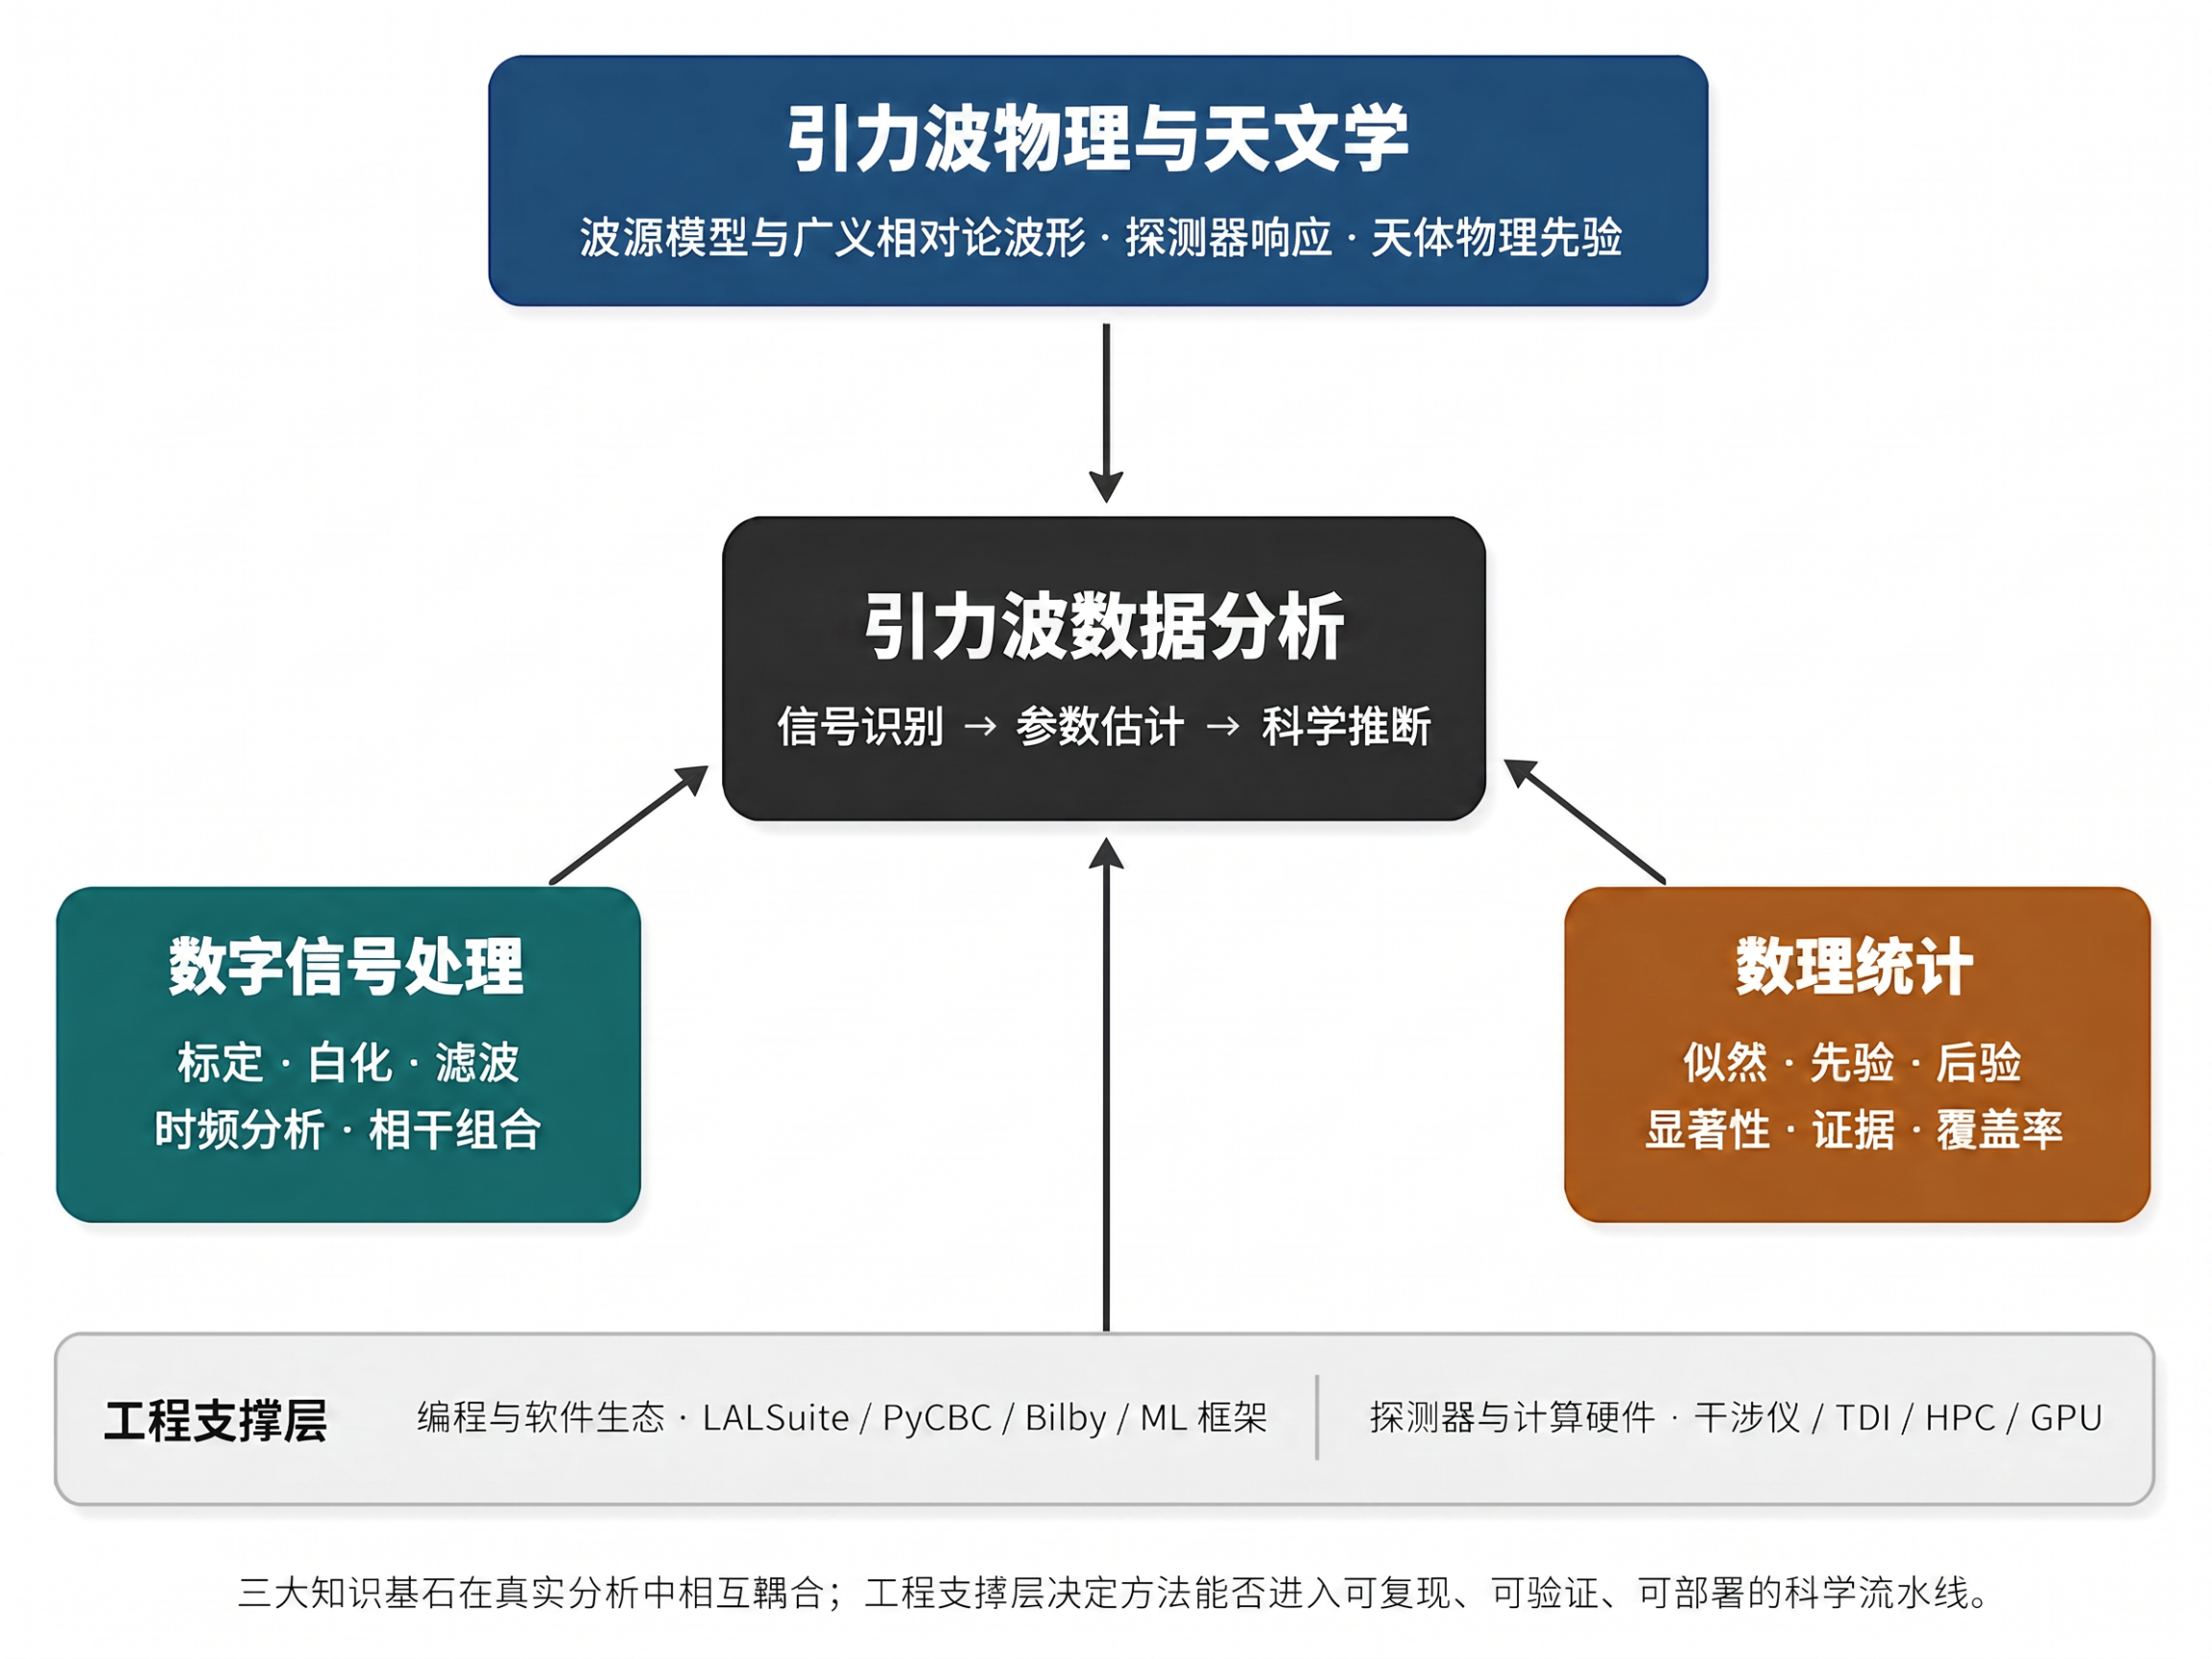
\includegraphics[width=0.92\textwidth]{figures/gw_knowledge_framework.png}
\caption{引力波数据分析的知识框架及其工程支撑。引力波物理与天文学、数字信号处理和数理统计构成三大知识基石，编程与软件生态、探测器与计算硬件构成工程支撑层；真实分析任务在三者交界处完成信号识别、参数估计和科学推断。}
\label{fig:gw_knowledge_framework}
\end{figure}

\textbf{核心创新点}包括以下五个方面：

其一，\textbf{物理驱动的网络设计}：感知层 CNN 将匹配滤波的物理先验以归纳偏置的形式嵌入网络结构（第5章），先验知识采样策略将物理先验转化为训练数据分布设计（第6章），两者共同构成“物理-数据融合”的早期实践。这一创新的核心洞察在于：引力波信号的物理特征（啁啾频率演化、特征时频轨迹、极化模式）可以通过网络结构设计而非仅靠数据学习来编码，从而在有限训练样本下实现更好的泛化性能，并赋予网络决策过程以物理可解释性。具体而言，MF-CNN 的感知层卷积核被初始化为匹配滤波模板的形状，使网络在训练初期就具备了物理意义明确的特征提取能力，而非从随机初始化出发盲目学习。

其二，\textbf{空间引力波参数估计的系统性突破}：归一化流和连续归一化流方法在太极任务的大质量双黑洞和极端质量比旋入参数估计中，实现比传统 MCMC 方法快几个数量级的推断速度（第6章），其中 EMRI 17 维参数空间的机器学习参数估计探索具有里程碑意义。传统的 MCMC 方法（如 Nested Sampling）对单个 EMRI 事件的参数估计需要大量波形计算，每次高保真波形计算可能耗时较长，总计算时间可达月级。归一化流方法通过一次性训练，将后验分布的采样时间压缩至秒级乃至更短时间尺度。这一加速不仅使低延迟参数估计成为可能，更为空间引力波全局拟合中的迭代优化提供了可行的计算基础。

其三，\textbf{Transformer 架构的引力波去噪}：WaveFormer 将自注意力机制引入引力波信号去噪，克服 CNN 的长程依赖局限（第7章）；针对空间探测器非稳态噪声的鲁棒去噪方法，为真实探测管道的构建提供了方法论基础。引力波信号的旋进阶段持续时间可达数分钟至数小时（对于低质量系统），信号的早期部分（低频、低振幅）与晚期部分（高频、高振幅）之间存在强烈的长程相关性——早期的频率演化速率决定了晚期的并合时刻，这种全局相关性是 CNN 等局部感受野方法难以有效捕捉的。Transformer 的自注意力机制天然适合处理这种长程依赖，WaveFormer 的实验结果表明，在相同参数量下，Transformer 架构的去噪性能显著优于 CNN，尤其在低信噪比条件下优势更为明显。

其四，\textbf{LLM 驱动的可解释算法自动发现}：Evo-MCTS 框架将大语言模型、蒙特卡洛树搜索与进化计算三者有机整合，在 MLGWSC-1 基准上超越强挑战赛基线 20.2\%，同时保持算法的物理可解释性（第8章）。这是 LLM 驱动的自动算法发现在引力波检测任务中的系统性实践。传统的神经架构搜索（NAS）和超参数优化方法通常将算法视为黑箱，优化目标是性能指标，而不关心算法的物理意义。Evo-MCTS 的创新在于：利用 LLM 的代码生成能力在算法空间中进行有意义的探索（而非随机变异），利用蒙特卡洛树搜索在算法演化树中进行有效的规划，利用进化计算维持算法多样性并避免局部最优。最终发现的算法不仅性能优越，而且其每一步操作都有明确的物理解释，可以被领域专家理解和验证。

其五，\textbf{方法论的跨领域普适性}：SBI 方法从引力波参数估计迁移到 21cm 森林宇宙学观测（第11章），beyond-GR 信号探测展示了 AI 作为理论无关探测器的潜力（第11章），共同指向 AI 方法在天文学中的更广泛应用前景。21cm 森林是高红移宇宙中性氢对背景射电源的吸收特征，其功率谱携带了宇宙再电离历史和暗物质性质的信息，但正向模拟极为耗时，传统的 MCMC 参数估计面临与引力波 EMRI 类似的计算瓶颈。将 SBI 方法迁移到这一领域，不仅解决了具体的计算问题，更验证了 SBI 作为通用推断框架的跨领域适用性，为 AI 方法在更广泛的天文学问题中的应用提供了方法论范本。

本书的组织结构遵循“问题驱动、方法递进、应用验证”的逻辑：第一、二部分建立理论基础和传统方法的参照系，第三、四部分系统介绍 AI 新方法及其与物理的融合，第五部分面向未来空间任务和发展趋势。每章均以具体的科学问题为起点，以定量的实验结果为支撑，以与全书论点的关联为收尾，形成完整的逻辑闭环。

表~\ref{tab:original_contributions}列出了与本书主题密切相关、作者参与完成的代表性研究工作。这些研究均依托具体合作团队开展，其中既包括作者主导或共同主导的工作，也包括作者作为合作者参与推进的重要成果；表中所称“贡献”指相关论文或项目对本书方法论主线的贡献，而非表示所有工作均为作者单独完成。

\begin{table}[htbp]
\centering
\caption{作者参与和合作完成的重要研究工作汇总}
\label{tab:original_contributions}
\small
\begin{tabular}{lllc}
\hline
\textbf{研究工作} & \textbf{核心贡献} & \textbf{对应章节} & \textbf{参考文献} \\
\hline
MF-CNN & 物理先验嵌入CNN，较早在真实LIGO-Virgo数据中系统应用 & 第5章 & \cite{wang2020deeplearning} \\
先验知识采样 & 物理先验引导的归一化流训练策略 & 第6章 & \cite{wang2022normflow} \\
太极归一化流 & 太极MBHB参数估计，处理时变响应函数 & 第6章 & \cite{du2024normflow} \\
CNF-MBHB & 流匹配CNF用于太极MBHB参数估计 & 第6章 & \cite{liang2024cnfmbhb} \\
CNF-EMRI & ML方法用于EMRI 17维参数估计探索 & 第6章 & \cite{liang2024cnfemri} \\
CVAE混合推断 & CVAE+贝叶斯精确协同，压缩至14\%时间 & 第6章 & \cite{sun2025cvae} \\
SBI综述 & SBI方法在引力波数据分析中的系统综述 & 第6章 & \cite{liang2026sbireview} \\
WaveFormer & Transformer架构引力波去噪 & 第7章 & \cite{wang2024waveformer} \\
长时序列去噪 & 30天旋近信号去噪与并合时刻预测 & 第7章 & \cite{xu2024denoising} \\
鲁棒去噪 & 非稳态噪声鲁棒深度学习去噪 & 第7章 & \cite{xu2024nonstationarty} \\
Evo-MCTS & LLM驱动自动算法发现，超越MLGWSC-1基线 & 第8章 & \cite{wang2025evomcts} \\
G-LNS & LLM引导大邻域搜索 & 第8章 & \cite{zhao2025glns} \\
Beyond-GR & AI作为理论无关引力波探测器 & 第11章 & \cite{wang2025beyondgr} \\
21cm SBI & SBI方法迁移至21cm森林宇宙学推断 & 第11章 & \cite{sun2025_21cm} \\
太极挑战综述 & 太极数据分析挑战与AI方法综述 & 第10章 & \cite{wang2024challenges} \\
\hline
\end{tabular}
\par\vspace{2mm}
\parbox{0.96\textwidth}{\zihao{-5}\textbf{说明：}本表仅用于说明这些合作研究与本书各章论述之间的对应关系。表中工作包含多位合作者和合作团队的共同贡献，具体作者排序、贡献分工和资助背景以相应论文原文为准。}
\end{table}

\section{本书章节安排}

本书共分五个部分、十二章，各章内容安排如下。

\textbf{第一部：理论基础与背景（第1--2章）}

第1章（绪论）系统梳理引力波天文学的历史脉络与探测现状，介绍地面和空间引力波探测器的技术特点与科学目标，分析数据分析面临的三层挑战（信号识别、参数估计、全局拟合），并概述本书的研究主题与五项核心创新点。

第2章（引力波信号与噪声建模）建立全书的物理与数学基础，系统介绍引力波波形模型（后牛顿近似、啁啾质量、SPA频域表示）、多类型引力波源的信号特征、探测器噪声的统计性质（功率谱密度、非高斯暂态、非平稳漂移），以及数据预处理的标准流程。

\textbf{第二部：传统方法与局限（第3--4章）}

第3章（经典的引力波数据分析方法）系统介绍匹配滤波与模板库构建、PyCBC/GstLAL 实际搜索流水线、贝叶斯推断与参数估计框架，以及蒙特卡洛采样方法的原理与实践挑战，并通过 MLGWSC-1 评测结果客观定位经典方法的性能边界。

第4章（高维参数空间与多模态挑战）从维度灾难、多源信号重叠、非平稳噪声三个维度定量分析经典方法在面向空间引力波探测器时的可扩展性瓶颈，为后续各章 AI 方法的引入提供清晰的问题动机。

\textbf{第三部：人工智能新方法（第5--7章）}

第5章（机器学习在引力波信号识别中的应用）以 MF-CNN 为核心，系统介绍卷积神经网络在引力波信号识别中的应用进展，包括感知层物理先验嵌入、集成学习、空间引力波多源统一检测、CNN 超参数调优、beyond-GR 信号探测，以及多角度可解释性分析。

第6章（生成模型与模拟推断）系统介绍模拟推断（SBI）的理论框架与主要变体（NPE/NRE/NLE），展示归一化流、连续归一化流（CNF）和混合推断策略在大质量双黑洞、极端质量比旋入参数估计中的系统应用，以及 SBI 方法向 21cm 森林宇宙学观测的跨领域迁移。

第7章（智能化信号分离与去噪）介绍 WaveFormer（Transformer 架构去噪）、长时旋近去噪与并合时刻预测、以及空间探测器非稳态噪声下的鲁棒信号提取，直接连接多信使天文学的实际预警需求。

\textbf{第四部：综合创新与融合（第8--9章）}

第8章（智能化启发式搜索与优化方法）介绍 LLM 驱动的自动算法发现方法演进（FunSearch→EoH→ReEvo→Evo-MCTS），重点展示 Evo-MCTS 在 MLGWSC-1 基准上超越强基线 20.2\% 的系统性验证，以及领域知识集成与可解释算法路径的关键作用。

第9章（物理驱动与数据驱动的融合方法）从互补缺陷分析出发，系统梳理物理先验嵌入、混合推断（精确协同）、可解释性验证三条融合路径，提出“精确协同”而非“近似替代”的方法论范式。

\textbf{第五部：前沿挑战与展望（第10--12章）}

第10章（未来空间引力波探测任务的数据挑战）以太极任务为主线，系统分析全局拟合的终极挑战、AI 方法在各类源分析中的分层角色、非稳态噪声的系统性处理，以及高保真仿真与真实探测管道的构建要素。

第11章（智能化引力波天文学的发展趋势）从四个维度展望 AI 在科学研究中角色的转变：LLM 驱动的自动算法发现、SBI 方法的跨领域迁移、AI 作为理论无关探测器，以及持续智能监测与人机协作的未来形态。

第12章（结语）以三条方法论主线（黑箱→可解释、近似替代→精确协同、单一方法→自动发现）总结全书贡献，并指出空间引力波全局拟合可行化、SBI 精度保证框架、AI 驱动科学发现泛化边界三个核心开放问题。

引力波天文学的独特地位在于，它是少数几个同时满足“物理理论极为精确”（广义相对论提供精确波形预言）和“信号检测极为困难”（应变灵敏度约$10^{-23}$）的科学领域，这一组合使它成为检验数据分析方法论的理想试验场：任何声称“有效”的方法都必须在极端噪声条件下通过严格的统计检验；任何声称“物理一致”的AI方法都可以通过对比理论预言来客观验证。这种近乎苛刻的科学标准，是引力波数据分析方法论研究的独特价值——在这里产生的方法论创新，往往具有超越引力波领域本身的普适性，因为它们是在最严格的科学标准下锻造出来的。

本书各章的内容组织遵循“从已知到未知、从经典到前沿、从单一到融合”的认知递进逻辑。第一部建立物理基础（读者需要的物理背景），第二部分析经典方法的能力与局限（为什么需要AI方法），第三部系统介绍AI新方法（怎么用AI方法），第四部展示融合与创新（怎么做到更好），第五部展望未来（下一步往哪里走）。这一逻辑链条不是线性阅读的约束，而是理解全书方法论体系的骨架。读者可以根据自己的知识背景选择合适的入口，但理解每章内容与整体框架的关联，是获得本书最大价值的关键。

\textbf{本书在线开源版本}已公开发布，欢迎在线阅读与交流：
\begin{center}
\url{https://iphysresearch.github.io/gwai-monograph/}
\end{center}
在线版与本书同步，支持全文检索和章节导航，并开放读者评论与勘误提交。

\section{本章小结}

本章从引力波天文学的历史脉络出发，系统梳理了从爱因斯坦1916年的理论预言到2015年 GW150914 首次直接探测的百年历程。Hulse-Taylor 脉冲双星 PSR B1913+16 的发现与轨道周期衰减的精密测量，提供了引力波存在的第一个间接证据，其与广义相对论预言的符合精度优于0.3\%，坚定了物理学界直接探测引力波的信心。LIGO 从1984年的构想到2002年初代运行、再到2015年 Advanced LIGO 的历史性突破，是科学史上长期愿景与技术攻关的典范。GW150914 的每一个观测细节——35至150 Hz 的啁啾频率演化、$10^{-21}$ 的峰值应变、7毫秒的两台探测器时延、5.1$\sigma$ 的统计显著性——都承载着深刻的物理意义，标志着引力波天文学新时代的开启。O1--O3 已公开近百个引力波候选事件，O4 进一步扩展样本规模；从 GW170817 的多信使天文学到 GW190521 的中间质量黑洞候选体，引力波天文学正在从“单次发现”迈向“海量统计”的大数据时代。

在探测器技术方面，Advanced LIGO 的臂腔（精细度约450，臂腔功率约750 kW）、信号循环腔、四级悬挂隔振系统和量子压缩光技术代表了当代精密测量的最高水平。下一代地面探测器（ET 的10公里三角形地下构型、CE 的40公里L型构型）将把灵敏度再提升一个量级，实现宇宙学距离上的引力波天文学。空间探测器（LISA、太极、天琴）将把探测窗口延伸至毫赫兹频段，探测超大质量黑洞并合、EMRI 和银河系双白矮星，三个任务的联合观测将大幅提升天空定位精度和参数估计精度。

在数据分析挑战方面，信号搜索面临极弱应变信号（典型量级 $\sim10^{-23}$）、非高斯 glitch（每小时数个至数十个）、非平稳噪声和高维参数空间（BBH 约15维，EMRI 约17维）的四重挑战；参数估计的科学价值体现在质量分布约束黑洞形成机制、自旋测量区分起源、距离测量给出哈勃常数等多个维度；空间引力波全局拟合的有效参数维度可达 $10^5$ 至 $10^7$ 量级，直接 MCMC 方法难以满足任务时效要求，是 AI 方法具有重要价值的根本动机。

本书的五项核心创新——MF-CNN 物理先验嵌入、SBI 参数估计加速、WaveFormer 智能去噪、Evo-MCTS 自动算法发现、物理-数据精确协同——均在这一问题框架下提出，构成了全书的方法论主线。理解这一框架，是把握后续各章具体方法动机的前提。

引力波天文学发展到今天，已经成为一门高度交叉的学科，其数据分析方法论的演进涉及广义相对论与天体物理学（物理建模）、统计学与贝叶斯推断（方法论基础）、信号处理与滤波（数据预处理）、机器学习与人工智能（方法革新）、以及高性能计算与软件工程（基础设施）。本书定位于方法论层面的系统梳理，不要求读者在所有五个方向都有深厚背景，但希望通过清晰的问题陈述和方法动机说明，帮助不同背景的读者在自己最熟悉的维度上理解本书的方法论贡献。对物理学家而言，重点是理解为何特定的物理先验对AI方法有决定性价值；对数学/统计学家而言，重点是理解引力波推断问题的特殊结构如何催生了SBI等新的推断范式；对计算机科学家而言，重点是理解科学约束如何重新定义了算法设计的目标和评估标准；对工程师而言，重点是理解从研究原型到生产系统的关键工程挑战。正是这种多维度的交叉融合，使引力波数据分析方法论成为科学AI方法论发展的最佳“试验场”之一。

\chapter{引力波信号与噪声建模}

引力波数据分析的所有方法——无论是传统的匹配滤波、贝叶斯推断，还是本书后续各章介绍的深度学习、模拟推断——都建立在对信号和噪声的数学描述之上。理解这些描述的物理基础，是理解后续方法选择的前提。本章系统介绍引力波信号的波形模型、源类型的多模态特征、探测器噪声的统计性质，以及数据预处理的标准流程。

\section{引力波的基本理论与波形模型}

在线性化广义相对论的弱场慢速近似下，引力波表现为时空度规的横波扰动~\cite{Einstein1916GW}。在横-无迹（TT）规范中，度规扰动为
\begin{equation}
  \mathrm{d}s^2 = -c^2\mathrm{d}t^2 + (\delta_{ij} + h_{ij}^{\mathrm{TT}})\,\mathrm{d}x^i\,\mathrm{d}x^j,
\end{equation}
其中 $h_{ij}^{\mathrm{TT}}$ 为引力波应变张量，其两个独立分量（$+$ 极化和 $\times$ 极化）描述了时空在垂直于传播方向平面内的伸缩和剪切。

\subsection{线性化广义相对论与引力波方程}

引力波的理论基础来自爱因斯坦广义相对论的线性化近似。爱因斯坦场方程的完整形式为
\begin{equation}
  G_{\mu\nu} = \frac{8\pi G}{c^4} T_{\mu\nu},
\end{equation}
其中 $G_{\mu\nu}$ 为爱因斯坦张量，$T_{\mu\nu}$ 为能量-动量张量。在弱场近似下，将时空度规写为闵可夫斯基度规加上小扰动：$g_{\mu\nu} = \eta_{\mu\nu} + h_{\mu\nu}$，其中 $|h_{\mu\nu}| \ll 1$。将此代入爱因斯坦方程并保留 $h_{\mu\nu}$ 的一阶项，得到线性化的场方程。

为简化方程，引入迹反转度规扰动 $\bar{h}_{\mu\nu} = h_{\mu\nu} - \frac{1}{2}\eta_{\mu\nu}h$（其中 $h = \eta^{\mu\nu}h_{\mu\nu}$ 为迹），并选取洛伦兹规范（Lorenz gauge）$\partial^\mu \bar{h}_{\mu\nu} = 0$，线性化场方程化为简洁的波动方程：
\begin{equation}
  \Box \bar{h}_{\mu\nu} = -\frac{16\pi G}{c^4} T_{\mu\nu},
\end{equation}
其中 $\Box = -\partial_t^2/c^2 + \nabla^2$ 为达朗贝尔算符。在真空中（$T_{\mu\nu} = 0$），此方程化为标准的波动方程 $\Box \bar{h}_{\mu\nu} = 0$，其解为以光速传播的横波——引力波。

在横-无迹（TT）规范中，通过进一步的规范选择，可以将引力波的独立自由度减少到最少。TT 规范要求 $h_{0\mu}^{TT} = 0$（时间分量为零）、$\partial^j h_{ij}^{TT} = 0$（横向条件）、$h_{ii}^{TT} = 0$（无迹条件）。在这一规范下，对于沿 $z$ 轴传播的引力波，度规扰动只有两个独立分量：
\begin{equation}
  h_{ij}^{TT} = \begin{pmatrix} h_+ & h_\times & 0 \\ h_\times & -h_+ & 0 \\ 0 & 0 & 0 \end{pmatrix} \cos(\omega t - kz),
\end{equation}
其中 $h_+$ 和 $h_\times$ 分别为两种极化模式的振幅。$h_+$ 极化描述沿 $x$-$y$ 轴方向的时空拉伸-压缩：当 $h_+ > 0$ 时，$x$ 方向拉伸、$y$ 方向压缩；当 $h_+ < 0$ 时反之。$h_\times$ 极化描述沿 $45°$ 方向的时空剪切。一个环形排列的自由质点在 $h_+$ 极化的引力波通过时，会交替地变形为沿 $x$ 方向拉长的椭圆和沿 $y$ 方向拉长的椭圆，形成特征性的“呼吸”运动。

\subsection{四极辐射公式与轨道衰减}

引力波的辐射功率由质量四极矩张量的时间导数决定。对于缓慢运动（$v \ll c$）的引力波源，辐射功率由四极公式给出：
\begin{equation}
  P = \frac{G}{5c^5} \left\langle \dddot{Q}_{ij} \dddot{Q}^{ij} \right\rangle,
\end{equation}
其中 $Q_{ij} = \int \rho(x_i x_j - \frac{1}{3}\delta_{ij}r^2)\,d^3x$ 为质量四极矩张量的无迹部分，上方三点表示对时间的三阶导数，尖括号表示对轨道周期的时间平均。这一公式揭示了引力波辐射的基本物理：只有质量分布的四极矩随时间变化才能辐射引力波，球对称或轴对称的运动（如球对称坍缩、均匀自转）不产生引力波辐射。

对于圆轨道双星系统，质量分别为 $m_1$ 和 $m_2$，轨道半径为 $r$，四极辐射功率为：
\begin{equation}
  P = \frac{32G^4}{5c^5} \frac{m_1^2 m_2^2 (m_1 + m_2)}{r^5}.
\end{equation}
这一功率来自轨道动能和引力势能的损失，导致轨道半径随时间减小（轨道衰减）。轨道衰减的速率为：
\begin{equation}
  \dot{r} = -\frac{64G^3}{5c^5} \frac{m_1 m_2 (m_1 + m_2)}{r^3},
\end{equation}
从初始轨道半径 $r_0$ 到并合（$r \to 0$）的时间尺度为 $\tau \propto r_0^4$。对于 Hulse-Taylor 脉冲双星 PSR B1913+16，轨道周期约7.75小时，轨道偏心率约0.617，理论预言的轨道周期衰减速率约为每年76微秒，与观测值的符合精度优于0.3\%，是引力波存在的最精确间接证据。

\subsection{后牛顿展开与引力波相位}

在旋进阶段，引力波波形的精确计算依赖后牛顿（post-Newtonian，PN）展开，即以 $v/c$（轨道速度与光速之比）为小参数的系统展开~\cite{Blanchet2014PN}。后牛顿展开的精度通常以 PN 阶数表示：$n$PN 阶对应 $(v/c)^{2n}$ 量级的修正。目前引力波数据分析中使用的波形模型通常精确到 3.5PN 阶（即 $(v/c)^7$ 量级），包含了质量比、对称质量比、自旋-轨道耦合、自旋-自旋耦合等多种修正项。

引力波相位的后牛顿展开在频域中具有特别简洁的形式。在驻相近似（SPA）下，频域波形的相位为：
\begin{equation}
  \Psi(f) = 2\pi f t_c - \phi_c - \frac{\pi}{4} + \frac{3}{128}(\pi \mathcal{M} f)^{-5/3} \sum_{k=0}^{7} \psi_k \left(\pi M f\right)^{k/3},
\end{equation}
其中 $t_c$ 为并合时刻，$\phi_c$ 为并合相位，$\mathcal{M}$ 为啁啾质量，$M = m_1 + m_2$ 为总质量，$\psi_k$ 为各阶后牛顿系数（依赖于质量比和自旋参数）。每个 $\psi_k$ 系数的精确值与引力理论相关，是检验广义相对论的探针：如果广义相对论在强场条件下存在偏差，这些系数将偏离广义相对论的预言值，从而在引力波相位中留下可测量的印记。

后牛顿展开的一个重要结论是啁啾质量 $\mathcal{M}$ 的主导地位：在最低阶（0PN）近似下，引力波频率演化完全由 $\mathcal{M}$ 决定，而与质量比无关。这意味着 $\mathcal{M}$ 是引力波信号中测量最精确的参数，其测量精度通常比单个天体质量高一到两个量级。对于 GW150914，$\mathcal{M} \approx 28.3\,M_\odot$ 的测量精度约为 $\pm 1.5\,M_\odot$（约5\%），而单个黑洞质量的测量精度约为 $\pm 4\,M_\odot$（约12\%）。

探测器测量的应变为
\begin{equation}
  h(t) = F_+(\alpha, \delta, \psi)\,h_+(t) + F_\times(\alpha, \delta, \psi)\,h_\times(t),
\end{equation}
其中 $F_+$、$F_\times$ 为天线响应函数，取决于源的天空位置 $(\alpha, \delta)$ 和极化角 $\psi$。

对于致密双星系统（双黑洞、双中子星），引力波波形由三个阶段组成：\textbf{旋近阶段}（inspiral）——两个天体在引力波辐射能量损失的驱动下螺旋靠近，频率单调增加，形成特征性的“啁啾”信号；\textbf{并合阶段}（merger）——两体系统的非线性动力学，需要数值相对论计算；\textbf{衰荡阶段}（ringdown）——并合后残余黑洞通过准简正模振荡辐射剩余能量，最终趋于稳态。

\begin{figure}[htbp]
\centering
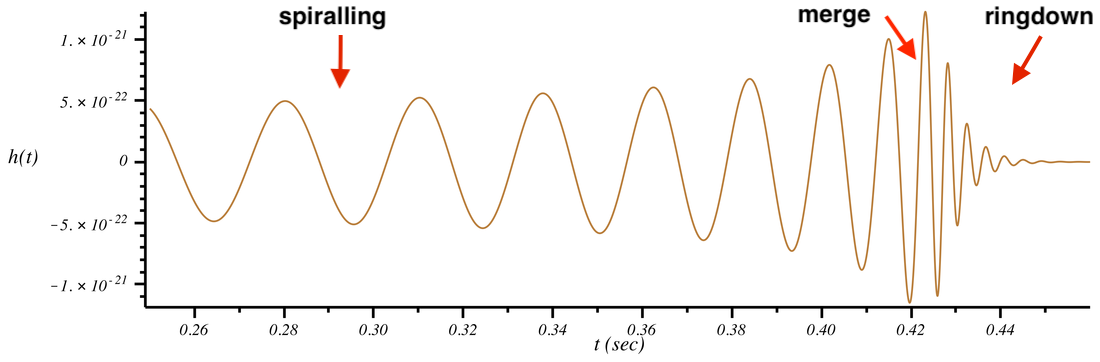
\includegraphics[width=0.96\textwidth]{figures/C2_gw_wf.png}
\caption{数值相对论波形模板在 Hanford（H1）观测站响应中的示意，对应 GW150914 型双黑洞并合事件。图中可见旋近（spiralling）、并合（merge）和衰荡（ringdown）三个阶段：频率与振幅在并合前快速增加，并合后残余黑洞以准简正模形式迅速衰减。该图引自文献资料中的 GW150914 波形模板示例~\cite{Abbott2016GW150914}。}
\label{fig:gw_waveform}
\end{figure}

实际应用中广泛使用的是现象学波形模型（IMRPhenomX 系列）和有效单体波形模型（EOBNR 系列），它们通过将后牛顿解析计算与数值相对论校准相结合，高效覆盖参数空间，构成匹配滤波模板库和贝叶斯参数估计的核心工具~\cite{Babak2017MCMC}。


\section{引力波源类型与多模态信号特征}

不同类型的引力波源在频率、持续时间、信号形态上存在显著差异，构成了信号空间的多模态结构。

\textbf{地面探测器频段（约 10 Hz--数千 Hz）}主要源类型包括：
\begin{itemize}
  \item \textit{双黑洞并合}（BBH）：最常见的观测事件类型，持续时间从数秒（高质量系统）到数分钟（低质量系统），信噪比通常较高。
  \item \textit{双中子星并合}（BNS）：持续时间更长（数分钟至数十分钟），并合后可能产生超新星和短伽马射线暴，是多信使天文学的核心目标。
  \item \textit{黑洞-中子星并合}（NSBH）：介于两者之间，若中子星被撕碎可能产生明显的电磁对应体。
\end{itemize}

\textbf{空间探测器覆盖的毫赫兹频段}的信号种类更为丰富：大质量双黑洞（$10^5$--$10^8\,M_\odot$）、极端质量比旋入（EMRI）、银河系双白矮星（数百万个同时叠加）、以及随机引力波背景。这种多源叠加的复杂性是空间引力波数据分析的核心挑战之一。

\subsection{双黑洞并合系统}

双黑洞并合（BBH）是迄今为止引力波探测中最常见的事件类型，GWTC-3 目录~\cite{Abbott2021GWTC3}中约90\%的事件为 BBH。BBH 的质量范围跨越多个量级：恒星级 BBH 的单个黑洞质量通常在 $5\,M_\odot$ 至 $100\,M_\odot$ 之间，总质量在 $10\,M_\odot$ 至 $200\,M_\odot$ 之间；中间质量 BBH（IMBHB）的质量在 $100\,M_\odot$ 至 $10^4\,M_\odot$ 之间，目前仅有少数候选体（如 GW190521，总质量约 $150\,M_\odot$，其主要成分约 $85\,M_\odot$ 落入对不稳定质量间隙）；大质量双黑洞（MBHB）的质量在 $10^4\,M_\odot$ 至 $10^9\,M_\odot$ 之间，是空间探测器（LISA/太极）的主要目标。

BBH 的形成机制是当前天体物理学的重要研究课题，主要有两类机制：孤立双星演化（isolated binary evolution）和动力学俘获（dynamical capture）。孤立双星演化机制认为，BBH 来自大质量双星系统的演化：两颗大质量恒星经历公共包层演化（common envelope evolution），轨道收缩，最终各自坍缩为黑洞，形成紧密的 BBH 系统。这一机制预言 BBH 的自旋通常与轨道角动量对齐（有效自旋参数 $\chi_\text{eff} > 0$），且质量比接近1（两个黑洞质量相近）。动力学俘获机制认为，BBH 在致密星团（球状星团、核星团）中通过引力散射形成：两个孤立黑洞在多体相互作用中被俘获为束缚系统。这一机制预言 BBH 的自旋方向随机（$\chi_\text{eff}$ 分布对称于零），且质量比分布更宽。

GWTC-3 的统计分析表明，观测到的 BBH 质量分布具有复杂结构，无法用单一的幂律分布描述：在约 $10\,M_\odot$ 处存在一个质量峰，在约 $35\,M_\odot$ 处存在另一个峰，在约 $3\,M_\odot$ 至 $5\,M_\odot$ 的“质量间隙”中存在若干候选体，在约 $50\,M_\odot$ 至 $130\,M_\odot$ 的“对不稳定质量间隙”中也有候选体（如 GW190521 的主要成分约 $85\,M_\odot$）。这些特征对黑洞形成机制提出了重要约束，也是引力波天文学与恒星演化理论交叉研究的核心问题。

\subsection{双中子星并合与多信使天文学}

双中子星并合（BNS）是引力波天文学中科学价值最丰富的事件类型之一。中子星的质量范围约为 $1.1\,M_\odot$ 至 $2.3\,M_\odot$，由核物质状态方程决定的最大质量约为 $2\,M_\odot$ 至 $3\,M_\odot$（具体值取决于状态方程）。BNS 的引力波信号持续时间远长于 BBH：对于典型的 $1.4+1.4\,M_\odot$ 系统，从进入 LIGO 灵敏频段（约10 Hz）到并合约需数分钟，在 Advanced LIGO 的灵敏频段内积累约 $10^4$ 个轨道周期，信号的相位演化携带了极为丰富的物理信息。

GW170817 是迄今唯一具有明确电磁对应体的引力波事件~\cite{Abbott2017GW170817}，其科学价值难以估量。该事件的引力波信号于2017年8月17日被 LIGO-Virgo 网络探测到，啁啾质量约为 $1.188\,M_\odot$，对应两颗中子星的质量约为 $1.17\,M_\odot$ 和 $1.60\,M_\odot$（在低自旋先验下），光度距离约为 $40^{+8}_{-14}$ Mpc，宿主星系为 NGC 4993。引力波信号结束约1.7秒后，Fermi 和 INTEGRAL 卫星探测到短伽马射线暴 GRB 170817A，强有力地支持了双中子星并合与一类短伽马射线暴之间的物理联系。此后数天至数周内，数十台光学、近红外、X射线、射电望远镜对 NGC 4993 进行了密集观测，发现了千新星（kilonova）AT2017gfo——这是重元素（如金、铂、铀）通过 r 过程核合成的重要观测证据，极大推进了宇宙重元素起源问题的研究。

BNS 并合后的产物是另一个重要的科学问题。根据并合前两颗中子星的总质量与最大中子星质量的关系，并合后可能形成：超大质量中子星（hypermassive neutron star，HMNS，寿命约数毫秒，最终坍缩为黑洞）、超稳定中子星（supramassive neutron star，寿命约数秒至数分钟或更长）、或直接坍缩为黑洞。GW170817 的后续电磁观测普遍支持其残余体在较短时间内坍缩为黑洞，但具体坍缩时刻和机制仍存在模型依赖与争议。未来的高频引力波探测（$\gtrsim 1$ kHz）将有望直接探测并合后残余体的振荡，为中子星状态方程提供更直接的约束。

\subsection{极端质量比旋入系统}

极端质量比旋入（EMRI）是空间引力波探测器最重要的科学目标之一，也是引力波数据分析中最具挑战性的问题。EMRI 系统由一个超大质量黑洞（质量 $M \sim 10^4$--$10^7\,M_\odot$）和一个轨道星体（质量 $\mu \sim 1$--$100\,M_\odot$，通常为中子星、白矮星或恒星级黑洞）组成，质量比 $q = \mu/M \sim 10^{-4}$--$10^{-7}$。

EMRI 的引力波信号具有极为丰富的物理内容。由于质量比极小，轨道星体对中心黑洞的反作用可以忽略，其轨道运动精确地追踪 Kerr 时空的测地线。在 LISA/太极的灵敏频段内，一个典型的 EMRI 事件在并合前约一年内会经历约 $10^5$ 个轨道周期，每次绕转产生的引力波相位变化与 Kerr 时空的几何精密相关。这意味着 EMRI 信号是对中心黑洞时空几何的极精密测绘：通过精确测量 EMRI 的引力波相位演化，可以以前所未有的精度测量中心黑洞的质量和自旋，检验“黑洞无毛定理”（即 Kerr 度规完全由质量和自旋描述），以及探测中心黑洞周围可能存在的暗物质晕或其他物质分布。

EMRI 信号的数据分析极为困难。首先，信号持续时间长（约一年），在频域中形成极为密集的谱线结构，与其他信号高度重叠。其次，EMRI 的参数空间约17维（中心黑洞质量和自旋、轨道星体质量、轨道偏心率、轨道倾角、初始相位等），且参数之间存在强简并。第三，高保真 EMRI 波形需要描述 Kerr 时空中的相对论轨道演化、引力辐射反作用和多谐波结构，计算代价远高于常规双黑洞波形。这些困难使得直接模板库搜索和常规逐点采样在 EMRI 问题中面临严峻压力，也使机器学习方法（特别是模拟推断）成为空间引力波数据分析中的重要候选路线。

\subsection{随机引力波背景}

随机引力波背景（SGWB）是由大量不可分辨的引力波源叠加形成的弥漫性背景辐射，类似于宇宙微波背景辐射（CMB）在引力波领域的对应物。SGWB 的来源可分为天体物理起源和宇宙学起源两大类。

天体物理起源的 SGWB 主要来自宇宙历史上所有双致密星并合事件的叠加。在地面探测器（LIGO/Virgo/KAGRA）频段，BBH 并合产生的背景能量密度约为 $\Omega_{GW} \sim 10^{-9}$（以临界密度为单位），目前尚未被探测到，但在 O4/O5 期间有望达到探测阈值。在 LISA 频段，银河系内不可分辨的双白矮星形成的混叠背景（confusion noise）是数据分析的主要挑战之一，其能量密度约为 $\Omega_{GW} \sim 10^{-11}$--$10^{-10}$，在 $1$--$10$ mHz 频段显著高于仪器噪声。

宇宙学起源的 SGWB 携带了宇宙早期历史的信息，是引力波宇宙学的核心目标。一阶宇宙相变（如电弱相变或 QCD 相变）产生的 SGWB 来自相变泡泡的碰撞和磁流体动力学湍流，其特征频率和能量密度取决于相变温度和强度，在 LISA 频段可能产生可探测的信号。宇宙弦（cosmic strings）产生的 SGWB 来自宇宙弦环的振荡和湮灭，其功率谱具有特征性的平坦形状，在宽频段内均有贡献。原初引力波（primordial gravitational waves）是宇宙暴胀期间产生的张量扰动，其功率谱由张量-标量比 $r$ 描述，目前的 CMB 观测给出 $r < 0.06$，对应的 SGWB 能量密度约为 $\Omega_{GW} \sim 10^{-16}$，远低于当前和近期探测器的灵敏度，但未来的空间探测器（如 BBO 或 DECIGO）有望探测到。

\textbf{SGWB 的探测方法}。SGWB 的探测面临独特的方法论挑战：背景信号本身是随机的，无法通过单次观测确认，必须通过统计方法从噪声中提取。标准方法是跨探测器互相关（cross-correlation）：对于两台探测器 $i$ 和 $j$，互相关统计量为
\begin{equation}
  \hat{C}_{ij}(f) = \frac{2}{T} \tilde{d}_i^*(f) \tilde{d}_j(f),
\end{equation}
其中 $T$ 为观测时间，$\tilde{d}$ 为频域数据。在高斯噪声假设下，$\hat{C}_{ij}$ 的期望值正比于 SGWB 的能量密度谱 $\Omega_{GW}(f)$，而噪声贡献在两台独立探测器之间不相关，因此通过长时间积分可以将信噪比提升至 $\text{SNR} \propto \sqrt{T}$。对于 LIGO 双探测器网络，探测 $\Omega_{GW} \sim 10^{-9}$ 的背景需要约一年的观测时间。

\textbf{AI 方法在 SGWB 分析中的应用}。传统互相关方法假设 SGWB 是各向同性的，但实际的天体物理背景（如 BBH 并合背景）可能具有各向异性，反映了宇宙大尺度结构的分布。深度学习方法可以通过学习背景信号的统计特征，在不假设各向同性的前提下提取 SGWB 的方向信息，这是传统方法难以实现的。此外，SBI 方法可以直接对 SGWB 的物理参数（如相变温度、宇宙弦张力）进行贝叶斯推断，绕过传统方法中对似然函数解析形式的依赖，为宇宙学参数约束提供更灵活的推断框架。

\textbf{脉冲星计时阵列（PTA）的纳赫兹背景}。2023年，多个脉冲星计时阵列（PTA）合作组——包括北美纳赫兹引力波天文台（NANOGrav）、欧洲脉冲星计时阵列（EPTA）、印度脉冲星计时阵列（InPTA）和帕克斯脉冲星计时阵列（PPTA）——相继报告了纳赫兹频段随机引力波背景的候选信号，其能量密度约为 $\Omega_{GW} \sim 10^{-9}$，频率约为 $10^{-9}$--$10^{-7}$ Hz。这一信号的物理起源尚不确定，候选解释包括超大质量双黑洞并合背景、宇宙弦网络、以及早期宇宙相变。PTA 的发现与 LISA/太极的毫赫兹频段观测形成互补，共同构成了多频段引力波宇宙学的观测基础。AI 方法在 PTA 数据分析中同样发挥着重要作用：机器学习方法被用于脉冲星计时残差的噪声建模、信号与噪声的分离，以及宇宙学参数的贝叶斯推断。

\subsection{银河系双星与混叠噪声}

银河系内存在约 $10^7$--$10^8$ 个双白矮星系统，其中大约 $10^4$ 个在 LISA/太极的灵敏频段（$1$--$10$ mHz）内可分辨，其余形成无法单独区分的“混叠噪声”背景。这一背景在低频段（$f \lesssim 3$ mHz）的能量密度高于仪器噪声，是空间引力波探测器数据分析的主要干扰源之一。

混叠噪声的统计特性与仪器噪声不同：它具有已知的频谱形状（由银河系双星种群的统计分布决定），且在银道面方向具有各向异性。这些特性使得混叠噪声既是科学目标（通过统计分析可以约束银河系双星种群的演化历史），也是数据分析的挑战（需要与仪器噪声和其他信号源同时建模）。

全局拟合框架（第10章）的核心任务之一，就是同时估计混叠噪声的统计参数和可分辨双星的物理参数，这要求在 $10^4$ 维以上的参数空间中进行联合贝叶斯推断。AI 方法——特别是 SBI 和快速参数估计方法——是使这一任务在计算上可行的关键技术支撑。

\section{探测器噪声性质}

探测器输出 $d(t) = h(t) + n(t)$ 中，噪声 $n(t)$ 的统计性质对数据分析方法的选择有决定性影响~\cite{Christensen2022noise}。

\textbf{功率谱密度（PSD）}是描述噪声频率特性的核心量：
\begin{equation}
  \langle\tilde{n}(f)\tilde{n}^*(f')\rangle = \frac{1}{2}S_n(f)\,\delta(f - f'),
\end{equation}
其中 $S_n(f)$ 为单边功率谱密度。在高斯平稳噪声假设下，$S_n(f)$ 完全描述了噪声的统计特性，匹配滤波在此假设下达到理论最优信噪比。

然而，真实探测器噪声远比高斯平稳假设复杂：

\textbf{非高斯成分}：探测器噪声中包含大量来自环境和仪器的暂态噪声（glitch），其幅度可比背景噪声高数个量级，持续时间从毫秒到数秒不等~\cite{Nuttall2018glitch}。glitch 的形态多样（“blip”、“koi fish”、“scattered light”等），统计上不满足高斯分布，是引力波搜索中误报率的主要来源。

\textbf{非平稳性}：探测器灵敏度随时间缓慢变化（“漂移”），在特定时段也会出现突发性的灵敏度下降~\cite{Buikema2020O3noise}。这要求数据分析算法能够实时估计和追踪噪声功率谱，而非使用固定的噪声模型。

\textbf{频谱线}：地面振动、电源频率（50/60 Hz 及其谐波）、悬挂系统共振等产生的窄带频谱线，在功率谱中形成锐峰，需要专门处理~\cite{Covas2018lines}。

\begin{figure}[htbp]
\centering
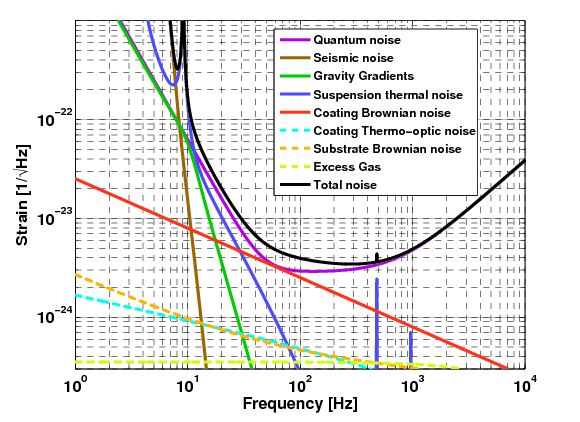
\includegraphics[width=0.82\textwidth]{figures/C2_ALIGO_broadband.png}
\caption{Advanced LIGO 中多种已知噪声来源对应的振幅谱密度。低频端主要受地震噪声、悬挂热噪声和重力梯度噪声限制，中频段由镜面与涂层热噪声等因素贡献，高频端则逐渐由量子噪声主导；黑色曲线表示各噪声项合成后的总噪声预算。图引自 Advanced LIGO 噪声预算资料，用于说明不同物理噪声源对探测器灵敏度曲线的分频段贡献~\cite{LIGOScientific2015detector}。}
\label{fig:noise_psd}
\end{figure}

量子散粒噪声（quantum shot noise）是地面引力波探测器高频灵敏度的根本限制，来源于光子计数的量子统计涨落。在相干态激光照射下，光子到达探测器的时间服从泊松分布，单位时间内的光子数涨落为 $\Delta N \sim \sqrt{N}$，对应的相位测量不确定度为 $\Delta\phi \sim 1/\sqrt{N}$。对于功率为 $P$ 的激光，单位时间内的光子数为 $N = P/(\hbar\omega)$，因此散粒噪声引起的应变噪声谱密度为：
\begin{equation}
  \sqrt{S_n^{shot}(f)} \propto \frac{1}{\sqrt{P_{circ}}} \cdot \frac{1}{L},
\end{equation}
其中 $P_{circ}$ 为臂腔内的循环光功率，$L$ 为臂长。这解释了为何 Advanced LIGO 要将臂腔功率提升至约750 kW——功率越高，散粒噪声越低。

与散粒噪声相对的是辐射压力噪声（radiation pressure noise）：高功率激光的光子动量涨落对镜面施加随机力，产生镜面位移噪声，其谱密度为：
\begin{equation}
  \sqrt{S_n^{rad}(f)} \propto \frac{\sqrt{P_{circ}}}{M f^2 L},
\end{equation}
其中 $M$ 为镜面质量。散粒噪声随功率增加而减小，辐射压力噪声随功率增加而增大，两者之积受海森堡不确定性原理约束，存在一个最优功率使总量子噪声最小——这就是标准量子极限（SQL）。在 SQL 处，散粒噪声与辐射压力噪声相等，总量子噪声为：
\begin{equation}
  \sqrt{S_n^{SQL}(f)} = \sqrt{\frac{8\hbar}{M(2\pi f)^2 L^2}}.
\end{equation}
突破 SQL 需要使用量子压缩光（squeezed light）技术：通过注入频率压缩态的真空场，可以在牺牲一个正交分量的不确定度的同时，降低另一个正交分量（相位或振幅）的不确定度，从而在特定频段将量子噪声降低至 SQL 以下。Advanced LIGO 在 O3 期间已成功实现约3 dB 的量子压缩，将高频灵敏度提升约40\%。

量子压缩光的物理机制需要更细致的说明。散粒噪声与辐射压力噪声在本质上来源于同一光场的量子涨落，两者的谱密度乘积受海森堡不确定性关系约束：$S_{shot}(f) \cdot S_{rp}(f) \geq \hbar^2/M^2L^2$，其几何均值即为标准量子极限处的总量子噪声。注入频率相关的压缩真空（frequency-dependent squeezed vacuum）可以对不同频率实现不同方向的压缩：在高频段（散粒噪声主导）压缩相位分量，在低频段（辐射压力噪声主导）压缩振幅分量。频率相关压缩需要一个滤波腔（filter cavity）来实现频率依赖的旋转角，Advanced LIGO 在 O4 运行中引入了长约300米的滤波腔，实现了频率相关压缩，在全频段量子噪声均低于 SQL。

在数据分析的视角下，量子噪声的优化与AI方法存在一个有趣的协同效应。量子压缩光降低散粒噪声的同时提升了高频灵敏度，这对高质量双黑洞并合（并合阶段频率$>100$ Hz）和双中子星合并（GW频率可达几kHz）的探测尤为重要。灵敏度提升后，在相同观测时间内可以探测到更远距离的事件，使引力波天文学的有效体积扩大，探测率相应提升。对数据分析算法而言，更高灵敏度意味着事件的平均信噪比更高，参数估计的精度更好；同时也意味着非高斯噪声（glitch）在高信噪比区域的相对贡献更大（因为真实信号变得更明显，而glitch的幅度分布不随探测器升级而改变）。这种“信号增强、glitch相对显眼”的效应，对机器学习方法的训练策略有直接影响：随着探测器升级，训练数据中的信噪比分布应相应调整，对高信噪比事件的训练权重可适当降低，同时加强对低信噪比但物理参数极端（如高质量比、高自旋）的事件的训练覆盖。这种“训练数据与探测器灵敏度协同演化”的策略，是AI方法在引力波领域持续保持高性能的关键工程实践。

从信息论角度理解量子极限：引力波探测本质上是测量两个检验质量之间的相对位移，这一测量行为不可避免地对被测系统施加反作用（辐射压力），这正是量子测量的反作用噪声。在标准量子力学框架下，任何不打破海森堡不确定性关系的测量方案都不能同时将位移分辨率和反作用力降至 SQL 以下。但通过“量子背作用规避”（quantum back-action evasion）技术——例如速度计方案（speed-meter）或变形探测器方案（variational readout）——可以在原理上规避辐射压力的反作用效应，从而使灵敏度突破 SQL。这类方案目前正在原型探测器上验证，未来的爱因斯坦望远镜（ET）和宇宙探测者（CE）计划引入这些技术，以期在全频段超越 SQL。

从实践角度，O3期间Advanced LIGO实现的约3 dB量子噪声降低，对应信噪比提升约$\sqrt{2}$倍，即灵敏度提升约40\%。这一提升意味着探测器对引力波事件的探测距离增加约26\%，对应探测体积增加约71\%（体积正比于距离的三次方）。从O2到O3期间，量子压缩的应用是引力波事件率从约10个/观测期增至约40个/观测期的重要技术因素之一，体现了量子光学技术在引力波天文学中的直接科学价值。

\subsection{热噪声与低温技术}

热噪声是地面引力波探测器中频段（约10至200 Hz）灵敏度的主要限制，来源于探测器各机械部件的热涨落。根据涨落-耗散定理，处于温度 $T$ 的机械系统的位移噪声谱密度为：
\begin{equation}
  S_x^{th}(f) = \frac{4k_B T}{\omega} \text{Im}[\chi(\omega)],
\end{equation}
其中 $\chi(\omega)$ 为系统的机械导纳（susceptibility），$\text{Im}[\chi(\omega)]$ 正比于机械损耗。这一公式揭示了降低热噪声的两条路径：降低温度 $T$，或降低机械损耗（提高机械品质因子 $Q$）。

Advanced LIGO 采用熔融石英（fused silica）纤维悬挂镜面，熔融石英在室温下的机械品质因子约为 $10^7$，是目前已知机械损耗最低的材料之一。镜面涂层（高反射率介质膜）的机械损耗是热噪声的主要来源，其品质因子约为 $10^4$，比基底低三个量级，是当前热噪声研究的核心问题。

KAGRA 采用了低温（约20 K）蓝宝石镜面，利用低温下材料机械损耗的显著降低来减小热噪声。蓝宝石在20 K 时的机械品质因子约为 $10^8$，比室温高约一个量级，理论上可将热噪声降低约3倍。低温技术的挑战在于：需要将约40公斤的镜面冷却至20 K，同时保持极低的振动水平，这需要专门设计的低温悬挂系统和辐射冷却方案。爱因斯坦望远镜（ET）计划采用约10 K 的硅镜面，将热噪声进一步降低约一个量级，使中频段灵敏度达到 $10^{-25}/\sqrt{\text{Hz}}$ 量级。

\subsection{重力梯度噪声与地下探测器}

重力梯度噪声（Newtonian noise，NN）是地面引力波探测器低频灵敏度的根本性限制，其物理机制与其他噪声源有本质区别：它不是通过机械耦合传递到检验质量，而是通过引力直接作用于检验质量，因此无法通过任何机械隔振手段消除。

重力梯度噪声的来源包括：地震波（P 波和 S 波）引起的地面密度涨落，在检验质量周围产生随时间变化的引力梯度；大气压力波（声波和重力波）引起的大气密度涨落，同样产生引力梯度；以及人类活动（车辆、机械振动）引起的局部密度涨落。在地面探测器的典型运行环境中，重力梯度噪声在约1至10 Hz 频段的贡献约为 $10^{-20}$--$10^{-19}\,\text{m}/\sqrt{\text{Hz}}$，远高于 Advanced LIGO 的设计灵敏度，是地面探测器低频截止（约10 Hz）的根本原因。

减小重力梯度噪声的主要方法有两种。第一种是在线减除（online subtraction）：在检验质量周围布置密集的地震传感器和气压传感器网络，实时测量引力梯度的涨落，然后从数据中减去其对检验质量位移的贡献。这一方法在理论上可将重力梯度噪声降低约一个量级，但实际效果受限于传感器的覆盖密度和测量精度。第二种是地下建设：将探测器建于地下数百米深处，利用岩层对地震波的天然衰减（约每100米衰减一个量级）来降低地震噪声，从而间接降低重力梯度噪声。爱因斯坦望远镜（ET）和 KAGRA 均采用了地下建设方案，ET 的设计深度约为100至200米，预计可将重力梯度噪声降低约两个量级，使低频截止降至约2至3 Hz。

\section{信号与噪声的数学建模方法}

引力波数据分析的标准内积定义为~\cite{Cutler1994PE}
\begin{equation}
  \langle a, b\rangle = 4\,\mathrm{Re}\int_0^\infty \frac{\tilde{a}(f)\tilde{b}^*(f)}{S_n(f)}\,\mathrm{d}f,
\end{equation}
这一定义使得在高斯平稳噪声下，$\langle n, n\rangle$ 服从 $\chi^2$ 分布，为统计检验提供了理论基础。

信号的最优信噪比（SNR）定义为
\begin{equation}
  \rho_\mathrm{opt} = \sqrt{\langle h, h\rangle} = \sqrt{4\int_0^\infty \frac{|\tilde{h}(f)|^2}{S_n(f)}\,\mathrm{d}f},
\end{equation}
它决定了特定信号在给定噪声背景下能够被探测到的理论极限。

在引力波参数估计中，贝叶斯似然函数的标准形式为~\cite{Veitch2015LALInference,Ashton2019Bilby}
\begin{equation}
  \ln p(d|\theta) = -\frac{1}{2}\langle d - h(\theta), d - h(\theta)\rangle + \text{const},
\end{equation}
这一表达式的计算需要对每个参数点 $\theta$ 生成波形 $h(\theta)$，是贝叶斯推断计算代价的主要来源。

\subsection{Fisher 信息矩阵与参数估计精度}

Fisher 信息矩阵（Fisher information matrix）是分析引力波参数估计精度的重要理论工具~\cite{Cutler1994PE}，它给出了在高信噪比极限下参数估计误差的理论下界（Cramér-Rao 界）。Fisher 矩阵定义为：
\begin{equation}
  \Gamma_{ij} = \left\langle \frac{\partial h}{\partial \theta_i}, \frac{\partial h}{\partial \theta_j} \right\rangle = 4\,\text{Re}\int_0^\infty \frac{\partial_i \tilde{h}(f) \cdot \partial_j \tilde{h}^*(f)}{S_n(f)}\,df,
\end{equation}
其中 $\partial_i = \partial/\partial\theta_i$ 为对第 $i$ 个参数的偏导数。Cramér-Rao 界给出参数估计误差的下界：
\begin{equation}
  \Delta\theta_i \geq \sqrt{(\Gamma^{-1})_{ii}},
\end{equation}
即参数 $\theta_i$ 的测量误差不能小于 Fisher 矩阵逆矩阵的对角元的平方根。在高信噪比极限下，贝叶斯后验分布趋近于以真实参数值为中心、协方差矩阵为 $\Gamma^{-1}$ 的多维高斯分布，Fisher 矩阵分析给出的精度估计与完整贝叶斯分析的结果一致。

Fisher 矩阵分析在引力波数据分析中有多方面的应用。首先，它揭示了哪些参数在高信噪比极限下最精确可测：对于双黑洞系统，啁啾质量 $\mathcal{M}$ 的 Fisher 矩阵元最大，对应最小的测量误差；而质量比 $q$ 和自旋参数的 Fisher 矩阵元较小，对应较大的测量误差。其次，Fisher 矩阵的非对角元揭示了参数之间的相关性（简并）：例如，距离 $d_L$ 和轨道倾角 $\iota$ 之间存在强简并（两者都影响信号振幅），导致单独测量这两个参数的精度远低于联合约束的精度。第三，Fisher 矩阵是匹配滤波模板库设计的理论基础：模板库的密度（即相邻模板之间的参数间距）由 Fisher 矩阵决定，确保任意真实信号与最近模板之间的匹配度不低于设计阈值。

需要注意的是，Fisher 矩阵分析在低信噪比条件下可能给出不准确的结果，因为贝叶斯后验分布在低信噪比时可能显著偏离高斯形状（出现多峰、长尾等非高斯特征）。对于实际的引力波参数估计，特别是对于信噪比较低的事件或参数空间中存在强简并的情况，需要使用完整的贝叶斯推断方法（如嵌套采样~\cite{Skilling2006nested}或 MCMC）来获得可靠的后验分布。标准推断工具 LALInference~\cite{Veitch2015LALInference} 和 Bilby~\cite{Ashton2019Bilby} 均实现了这些方法。

Fisher 矩阵在引力波参数估计中的具体应用价值可以通过一个典型的双黑洞系统来具体说明。对于总质量约为 $60\,M_\odot$、SNR约为20的双黑洞并合事件，Fisher 矩阵分析给出各参数的理论精度估计如下：啁啾质量 $\mathcal{M}$ 的相对误差约为 $\Delta\mathcal{M}/\mathcal{M} \approx 0.05\%$，这对应的物理约束（质量精度约 $0.03\,M_\odot$）远超任何其他类型的黑洞质量测量手段；质量比 $q = m_1/m_2$ 的相对误差约为 $\Delta q/q \approx 15\%$，这是因为质量比对波形相位演化的贡献从1.5PN阶才开始显现，而啁啾质量在0PN阶就主导了相位演化，因此 Fisher 矩阵中质量比对应的对角元远小于啁啾质量。

参数间相关性（简并结构）的分析同样是 Fisher 矩阵的重要应用。$\Gamma$ 矩阵的非对角元素 $\Gamma_{ij}$ 反映了参数 $\theta_i$ 和 $\theta_j$ 之间的信息耦合强度。在双黑洞系统中，以下几对参数表现出显著的相关性：（1）啁啾质量 $\mathcal{M}$ 与并合时刻 $t_c$ 之间的负相关（$\Gamma_{\mathcal{M},t_c} < 0$），因为较重的系统旋进更快，等效于较晚的“有效并合时刻”；（2）有效自旋参数 $\chi_{eff} = (m_1\chi_{1z} + m_2\chi_{2z})/(m_1+m_2)$ 与质量比 $q$ 之间的强正相关，原因在于两者对引力波相位演化的贡献在后牛顿展开中有部分重叠（均在1.5PN阶出现），这一简并被称为“质量-自旋简并”，是精确测量黑洞自旋的根本障碍；（3）光度距离 $d_L$ 与轨道倾角 $\iota$ 之间的强相关，两者都通过波形振幅的角度因子 $F(1+\cos^2\iota)/2$ 和 $F\cos\iota$ 影响信号强度，对于单探测器观测，两者几乎完全简并（Fisher 矩阵对应子块接近奇异），多探测器网络可以通过方向图差异部分解除这一简并。

Fisher 矩阵分析揭示的参数简并结构，是理解 SBI 方法为何选择特定网络架构的物理基础。第6章介绍的归一化流方法之所以能够高效建模引力波参数后验，部分原因在于其非线性变换能力可以适应 Fisher 矩阵所揭示的弯曲等值线结构——归一化流的每一层变换对应于对后验流形的逐步展开，最终将复杂的简并后验变换为接近正态的基础分布。

Fisher矩阵分析的另一个重要应用是指导多探测器网络的优化设计。对于$N$个探测器组成的网络，联合Fisher矩阵为各探测器Fisher矩阵之和，$\Gamma^{net} = \sum_{k=1}^N \Gamma^{(k)}$，其逆矩阵给出联合参数估计的精度。通过分析 $\Gamma^{net}$ 的特征值和特征向量，可以识别哪些参数方向是“信息充足”的（大特征值，对应精确可测的参数组合），哪些是“信息缺乏”的（小特征值，对应难以约束的参数方向）。对于天空定位参数 $(\alpha, \delta)$，Fisher矩阵分析表明，三探测器（H1+L1+V1）配置相比双探测器（H1+L1）的天空定位精度提升约5-10倍，因为第三台探测器打破了双探测器配置下天空位置的环状简并。这一结论不仅验证了Virgo探测器在LIGO-Virgo网络中的重要性，也指导了未来全球引力波探测器网络（加入LIGO-India、KAGRA等）的布局优化。在AI参数估计方法的训练中，Fisher矩阵分析可以用于指导训练数据的设计：对于Fisher矩阵揭示的高度简并参数方向，需要在训练集中引入更多样化的样本来覆盖简并流形，而非简单的均匀采样。

白化（whitening）是引力波数据分析中最基本的预处理操作，其数学本质是将有色噪声转化为白噪声，从而简化后续的统计分析。白化操作定义为：
\begin{equation}
  \tilde{d}_w(f) = \frac{\tilde{d}(f)}{\sqrt{S_n(f)/2}},
\end{equation}
其中 $S_n(f)/2$ 为双边功率谱密度。白化后的噪声 $\tilde{n}_w(f)$ 满足 $\langle \tilde{n}_w(f) \tilde{n}_w^*(f') \rangle = \delta(f-f')$，即为单位白噪声。

白化操作的重要性在于它建立了频域内积与时域 $L^2$ 内积之间的等价关系。在白化后的数据中，标准内积退化为简单的频域向量内积：
\begin{equation}
  \langle a, b \rangle = 4\,\text{Re}\int_0^\infty \frac{\tilde{a}(f)\tilde{b}^*(f)}{S_n(f)}\,df = 2\int_{-\infty}^{\infty} \tilde{a}_w(f)\tilde{b}_w^*(f)\,df = 2\int_{-\infty}^{\infty} a_w(t)b_w(t)\,dt,
\end{equation}
其中最后一步利用了 Parseval 定理。这一等价性意味着：在白化后的数据上，匹配滤波等价于简单的时域互相关，计算效率大幅提升。

对于深度学习方法，白化是几乎所有方法的必要预处理步骤。未经白化的原始数据在低频段（$\lesssim 30$ Hz）的噪声功率比高频段高出数个量级，如果直接输入神经网络，网络将被低频噪声主导，无法有效学习引力波信号的特征。白化后，不同频率的噪声贡献归一化，网络可以均等地关注所有频率的信号特征，从而实现更好的学习效果。此外，白化还使得网络的输入分布更接近标准正态分布，有利于梯度下降的收敛。

\section{数据预处理与特征提取}

原始探测器数据在进入分析流程前通常需要经过若干预处理步骤~\cite{Buikema2020O3noise}。

\textbf{白化}（whitening）：将数据除以噪声功率谱的平方根，使不同频率的噪声贡献归一化。白化是几乎所有深度学习方法的必要预处理步骤，确保网络不会被低频噪声主导。

\textbf{带通滤波}：滤除探测器灵敏频段之外的噪声，通常与白化结合使用。

\textbf{时频变换}：Q 变换（Q-transform）和连续小波变换（CWT）将时域数据转换为时频图，直观展示信号的时频演化特征，常用于可视化和深度学习的输入表示。

\textbf{glitch 处理}：对已知类型的 glitch 可以进行减除或标记（gating），以降低其对后续分析的影响。这一步骤在实际数据分析中至关重要，但在方法研究中常被简化处理。

\subsection{Q 变换与时频分析}

Q 变换（Q-transform）是引力波数据分析中最常用的时频分析工具，其数学定义为：
\begin{equation}
  X(t, f; Q) = \int_{-\infty}^{\infty} d(t') \, w(t'-t, f, Q) \, e^{-2\pi i f t'} \, dt',
\end{equation}
其中 $w(t, f, Q)$ 为高斯窗函数：
\begin{equation}
  w(t, f, Q) = \left(\frac{\pi Q^2}{2}\right)^{1/4} \frac{1}{\sqrt{f}} \exp\left(-\frac{\pi^2 Q^2 t^2}{f^2}\right) \exp\left(-\frac{Q^2}{4}\right),
\end{equation}
$Q$ 参数（品质因子）控制时频分辨率的权衡：$Q$ 值越大，频率分辨率越高但时间分辨率越低；$Q$ 值越小，时间分辨率越高但频率分辨率越低。这一权衡由海森堡不确定性原理决定：$\Delta t \cdot \Delta f \geq 1/(4\pi)$。

Q 变换的优势在于其对数频率轴的自然适应性：引力波信号的频率演化在对数频率轴上更为均匀，Q 变换在对数频率轴上具有恒定的相对频率分辨率 $\Delta f/f = 1/Q$，因此能够在宽频段内均匀地捕捉信号特征。在实际应用中，通常选择 $Q$ 值在5至100之间，并对多个 $Q$ 值的结果取最大值，以同时保留时间和频率分辨率。

Q 变换在引力波数据分析中有多种应用。在可视化方面，Q 变换时频图是引力波信号最直观的表示方式：BBH 并合的啁啾信号在 Q 变换图上呈现为从低频到高频的弧形轨迹，频率随时间单调增加，振幅在并合时刻达到峰值；glitch 在 Q 变换图上通常呈现为局部的亮斑或条纹，形态与引力波信号有明显差异。在机器学习方面，Q 变换时频图常被用作卷积神经网络（CNN）的输入，利用 CNN 对图像特征的强大提取能力来识别引力波信号和分类 glitch。Gravity Spy 项目就是利用 CNN 对 Q 变换图进行分类，实现了 glitch 的自动化识别和分类，大幅减轻了人工标注的工作量。

\subsection{数据质量控制与 glitch 处理}

数据质量控制（data quality，DQ）是引力波数据分析流水线的重要组成部分，其目标是识别和标记探测器数据中的质量问题，为后续分析提供可靠的数据段。

数据质量控制的第一层是在线监测：在探测器运行期间，数百个辅助通道（auxiliary channels）持续监测探测器的各个子系统（激光功率、镜面位置、环境传感器等）。当某个辅助通道出现异常时，数据质量系统会自动生成一个“数据质量标记”（DQ flag），标记该时段的数据可能受到特定噪声源的污染。这些标记分为不同的类别（Category 1、2、3），对应不同程度的数据质量问题，分析人员可以根据科学目标选择是否排除这些时段。

数据质量控制的第二层是离线分析：在数据采集后，通过时频图的视觉检查和自动化算法来识别 glitch。视觉检查由人工完成，但随着数据量的增加，人工检查已无法满足需求，因此发展了多种自动化方法。Omicron 算法基于 Q 变换，通过在时频图中寻找超过阈值的局部极大值来识别 glitch，并给出每个 glitch 的时间、频率、持续时间和信噪比等参数。Gravity Spy 项目利用卷积神经网络对 Omicron 识别的 glitch 进行分类，将其归入约20种已知类型，并通过主动学习（active learning）循环持续改进分类器的性能。

glitch 的处理方法主要有三种。第一种是门控（gating）：在时域中将包含 glitch 的时段乘以一个平滑的窗函数，将 glitch 的贡献降至零，然后用零填充或插值替代。门控简单有效，但会损失该时段的数据，且可能引入边缘效应。第二种是减除（subtraction）：利用辅助通道的信息，建立 glitch 的物理模型，然后从主通道数据中减去 glitch 的贡献。这一方法可以在不损失数据的情况下降低 glitch 的影响，但需要精确的 glitch 模型，实现难度较高。第三种是统计鲁棒化：在数据分析算法中引入对非高斯噪声的鲁棒性，例如使用重尾分布（如学生 t 分布）替代高斯分布作为噪声模型，或使用基于排名的统计量替代基于均值的统计量。这些方法不需要显式识别和处理 glitch，而是通过算法设计来降低 glitch 对分析结果的影响，是机器学习方法在引力波数据分析中的重要研究方向之一。

这些预处理步骤构成了引力波数据分析管道的第一层，其质量直接影响后续所有方法的性能。本书后续章节介绍的各种 AI 方法，均在预处理后的数据上运行。需要注意的是，真实流水线并非简单的“白化—滤波—分类”线性流程：标定、探测器表征、数据质量审查、搜索触发、事件验证和参数估计之间存在反馈关系，辅助通道和环境传感器也持续参与候选事件的可信度评估。

\begin{figure}[htbp]
\centering
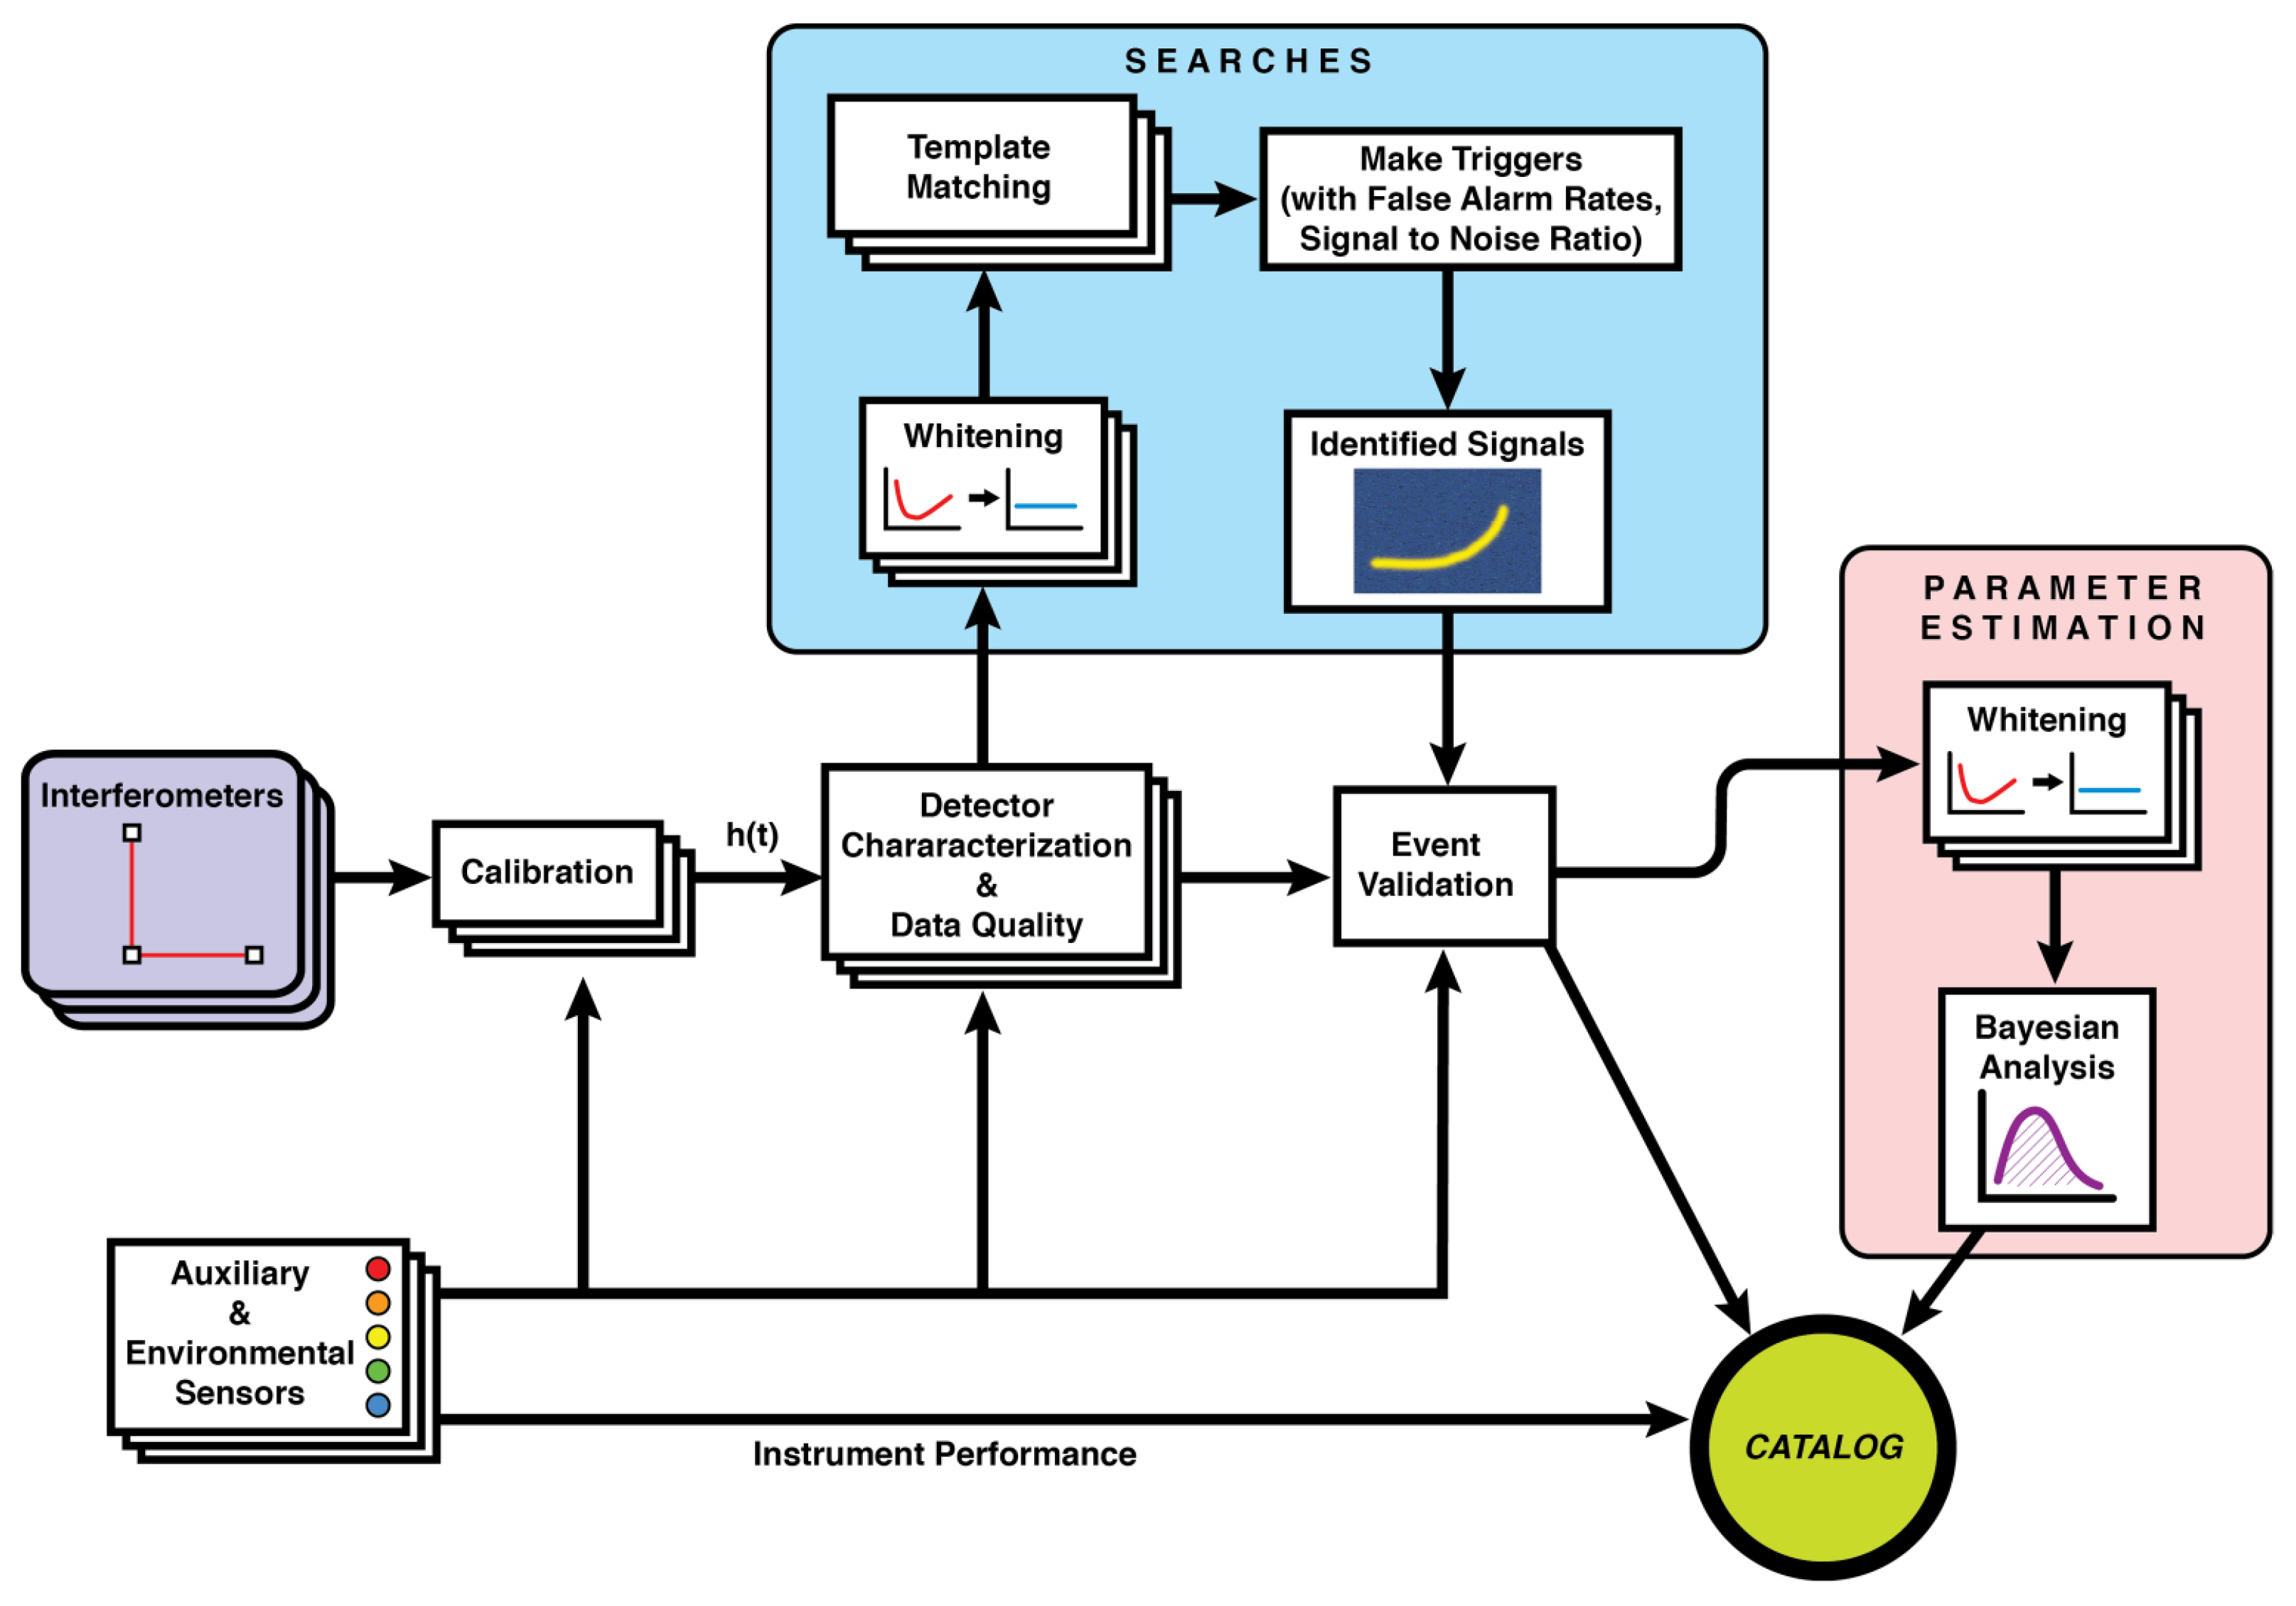
\includegraphics[width=0.98\textwidth]{figures/galaxies-10-00012-g001.png}
\caption{地面引力波数据分析与探测器表征的实际工作流示意。干涉仪数据经标定得到应变时间序列 $h(t)$，并与辅助通道、环境传感器和数据质量信息共同进入搜索、事件验证和参数估计流程；最终可靠候选事件进入引力波事件目录。图引自 Davis 与 Walker 对地面引力波探测器表征和噪声缓解工作的综述~\cite{Davis2022DetectorCharacterization}。}
\label{fig:pipeline}
\end{figure}

\begin{table}[htbp]
\centering
\caption{Advanced LIGO 主要噪声源特性对比}
\label{tab:noise_sources}
\small
\begin{tabular}{lcccc}
\hline
\textbf{噪声类型} & \textbf{主导频段} & \textbf{物理机制} & \textbf{降低方法} & \textbf{典型量级} \\
\hline
量子散粒噪声 & $\gtrsim 200$ Hz & 光子计数泊松涨落 & 提高激光功率、压缩光 & $4\times10^{-24}/\sqrt{\text{Hz}}$ \\
辐射压力噪声 & $\lesssim 50$ Hz & 光子动量涨落 & 增大镜面质量 & $10^{-23}/\sqrt{\text{Hz}}$ \\
热噪声（镜面） & 20--200 Hz & 布朗运动 & 低温、高Q材料 & $10^{-23}/\sqrt{\text{Hz}}$ \\
热噪声（悬挂） & 10--50 Hz & 悬丝热涨落 & 熔融石英纤维 & $10^{-23}/\sqrt{\text{Hz}}$ \\
地震噪声 & $\lesssim 10$ Hz & 地面振动 & 主动隔振系统 & $10^{-21}/\sqrt{\text{Hz}}$ \\
重力梯度噪声 & $\lesssim 10$ Hz & 引力直接耦合 & 地下建设、传感器减除 & $10^{-21}/\sqrt{\text{Hz}}$ \\
频谱线 & 离散频率 & 电源、机械共振 & 陷波滤波器 & 局部超出 $10\times$ \\
\hline
\end{tabular}
\end{table}

引力波数据预处理的每一步都有其不可忽视的物理动机，理解这些动机是正确实施预处理的关键。白化操作消除了噪声PSD的频率依赖性，使各频率分量的噪声贡献归一化——这一步骤对于深度学习方法尤为关键，因为神经网络如果直接处理非白化数据，其训练过程将被低频大噪声所主导，导致网络对低频引力波特征不敏感。带通滤波则利用了引力波信号频段的物理先验：引力波信号主要集中在探测器灵敏频段（地面探测器约20-1000 Hz），带通滤波在保留信号的同时去除灵敏频段以外的噪声成分，相当于在预处理层面已经利用了物理知识。Q变换的时频表示为机器学习方法提供了直观且信息丰富的输入格式：引力波的啁啾特征在Q变换时频图上表现为清晰的“上弯曲线”，这种直观特征既便于人工识别，也使CNN能够通过卷积操作高效提取。

从系统工程角度，数据预处理流水线的设计需要在物理严格性和计算效率之间取得平衡。对于在线（实时）引力波搜索，每一步预处理都必须在严格的时间约束下完成——通常要求整个预处理流水线在信号到达后1-2秒内完成，以便后续的触发判断和多信使预警。这一约束限制了预处理步骤的复杂程度：可以使用的噪声PSD估计窗口通常为4-256秒（而非更长时间的精确估计），白化滤波器的时域长度受限，Q变换的参数也需要在精度和速度之间折中。理解这些工程约束，对于在实际引力波数据分析流水线中部署AI方法时做出合理的设计选择，是不可缺少的背景知识。

引力波数据预处理方法本身也在持续发展中。传统的Welch方法（使用历史数据的段平均估计噪声PSD）在噪声平稳时表现良好，但在噪声突变时（如仪器状态改变后）需要一段时间才能重新收敛，导致过渡期内的白化质量下降。基于机器学习的噪声估计方法——如使用LSTM或Transformer追踪噪声PSD的时间演化——可以更快速地适应噪声变化，预计在下一代探测器（Einstein Telescope、Cosmic Explorer）的噪声管理中发挥重要作用。类似地，glitch的实时处理方法也在从“事后减除”向“实时抑制”演进：深度学习去噪方法（第7章）可以在数据产生后毫秒内完成glitch的识别和部分减除，为后续的匹配滤波提供更干净的输入数据。这种“AI预处理+经典分析”的流水线架构，是未来引力波数据分析基础设施的重要发展方向，也是物理-数据融合（第9章）在系统层面的具体体现。

噪声功率谱密度的精确估计对引力波参数估计的精度有直接影响。在贝叶斯参数估计中，引力波似然函数 $\ln p(d|\theta) = -\frac{1}{2}\langle d-h(\theta), d-h(\theta)\rangle$ 中的内积依赖于PSD作为噪声权重；若PSD估计存在偏差，则似然函数值将系统性偏离真实值，导致参数后验分布偏移。这一效应在低信噪比事件（$\rho < 12$）中尤为显著，因为PSD估计的相对误差与SNR成反比地影响后验的偏移量。LIGO标准分析流程使用BayesLine算法对每个候选事件进行精细的PSD估计，将PSD不确定度作为额外的贝叶斯自由度纳入参数估计框架，从而减轻PSD估计误差对参数精度的影响。深度学习方法在处理这一问题时具有独特优势：通过在训练数据中引入不同PSD条件的模拟，网络可以隐式地学习对PSD不确定性的鲁棒性，而无需显式地建模PSD不确定度——这是深度学习的“隐式正则化”特性在数据预处理环节的具体体现。

本章系统建立了引力波数据分析的物理与数学基础，为后续各章的方法介绍提供了完整的理论框架。

在引力波基本理论方面，从爱因斯坦场方程的线性化出发，推导了引力波的波动方程和 TT 规范下的极化描述，阐明了四极辐射公式和轨道衰减机制，并系统介绍了后牛顿展开的物理内容和频域 SPA 波形表示。啁啾质量作为引力波信号中测量最精确的参数组合，其主导地位来自后牛顿展开的最低阶项，是匹配滤波和参数估计的核心工具。

在引力波源类型方面，地面探测器对应的高频窗口与 LISA/太极/天琴覆盖的毫赫兹窗口共同构成了多模态信号空间。BBH 的质量分布复杂结构（约 $10\,M_\odot$ 和 $35\,M_\odot$ 处的峰值、质量间隙中的候选体）对黑洞形成机制提出了重要约束；GW170817 的多信使观测揭示了双中子星并合是短伽马射线暴和千新星的起源；EMRI 的精密相位演化是对 Kerr 时空几何的极精密测绘；随机引力波背景携带了宇宙早期历史的信息。空间探测器的多源叠加特性（数百万个信号同时存在）是全局拟合问题的根本来源。

在噪声建模方面，功率谱密度 $S_n(f)$ 是描述噪声频率特性的核心量，量子散粒噪声、热噪声和重力梯度噪声分别主导高频、中频和低频段。真实探测器的非高斯暂态（glitch）和非平稳漂移使高斯平稳假设在实践中受到严峻挑战，是引力波搜索中误报率的主要来源。标准量子极限（SQL）和量子压缩光技术代表了量子噪声控制的前沿，低温技术（KAGRA、ET）是降低热噪声的根本途径，地下建设是突破重力梯度噪声限制的必要选择。

在数学建模方面，标准内积定义、最优 SNR 公式和贝叶斯似然函数构成了后续所有方法的数学基础。Fisher 信息矩阵给出了参数估计精度的理论下界，揭示了参数简并的结构，是模板库设计的理论依据。白化操作建立了频域内积与时域 $L^2$ 内积的等价关系，是深度学习方法的必要预处理步骤。Q 变换提供了引力波信号的直观时频表示，数据质量控制和 glitch 处理是保证分析可靠性的重要环节。这些基础工具和概念将贯穿本书后续各章，是理解 AI 方法设计选择的物理基础。

\section{本章小结}

本章建立了引力波数据分析的物理与数学基础。在信号模型方面，TT规范下的度规扰动和天线响应函数描述了探测器的测量原理，IMRPhenomX和EOBNR等现象学波形模型覆盖了旋进-并合-衰荡的完整波形，构成模板库和参数估计的核心工具。在源类型方面，地面探测器对应的高频窗口与 LISA/太极/天琴覆盖的毫赫兹窗口构成了多模态信号空间，其中空间探测器的多源叠加特性是数据分析的核心挑战。在噪声建模方面，功率谱密度$S_n(f)$是描述噪声频率特性的核心量，而真实探测器的非高斯暂态（glitch）和非平稳漂移使高斯平稳假设在实践中受到严峻挑战。标准内积定义、最优SNR公式和贝叶斯似然函数构成了后续所有方法的数学基础，白化、带通滤波、Q变换等预处理步骤则是数据进入分析流程的必要前提。
